% =====================================================================
% AMMPER-2 --- SUPPLEMENTARY MATERIAL (STANDALONE DOCUMENT)
%
% This file is self-contained: compile it directly, independently of
% main.tex and of the ASM class.
%
%   pdflatex supplementary
%   bibtex   supplementary
%   pdflatex supplementary
%   pdflatex supplementary
%
% It deliberately does NOT use asmarticle.cls (the ASM class is designed
% for the main article body and mangles a separately submitted supplement).
% Required packages are all standard TeX Live: graphicx, subcaption,
% amsmath, amssymb, geometry, url, natbib.
%
% CONTENTS POLICY: this supplement contains only material that is
% explicitly called out from the main text. Every figure below (S1-S7) is
% cited in main.tex, and each supplementary text section names the main-text
% section that defers to it. Derivations that merely duplicated the main-text
% Materials and Methods were removed.
%
% FIGURE NUMBERING: \thefigure is renewed to S\arabic{figure}, so the figure
% environments below render as S1, S2, ... in source order and every \label is
% named for the number it actually receives. Check both when inserting a figure:
% a \label whose name disagrees with its rendered number is invisible in the PDF
% but silently misdirects every callout in main.tex.
% =====================================================================
\documentclass[11pt]{article}

\usepackage[letterpaper,margin=1in]{geometry}
\usepackage[T1]{fontenc}
\usepackage[utf8]{inputenc}
\usepackage{amsmath}
\usepackage{amssymb}
\usepackage{graphicx}
\usepackage{subcaption}
\usepackage{url}
\usepackage[numbers,square,comma]{natbib}

\graphicspath{{./}{Figures/}{Panels/}}

% Number everything with an "S" prefix, per journal convention.
\renewcommand{\thefigure}{S\arabic{figure}}
\renewcommand{\theequation}{S\arabic{equation}}

\setlength{\parskip}{0.4em}
\setcounter{secnumdepth}{0}   % headings are unnumbered, as in the main text

\begin{document}

\begin{center}
{\Large\bfseries Supplementary Material}
\end{center}

\vspace{1em}

% =====================================================================
% SUPPLEMENTARY TEXT
% =====================================================================
\section{Supplementary text}

\subsection{S1. Multivariate distribution used for ROS diffusion}
\label{sec:ros-distribution}

\textit{Corresponds to Materials and Methods, ``Diffusion and decay ROS molecule
modeling'' in the main text, where this section is cited.}

When an ionizing radiation path is created in AMMPER using RITRACKS, a radiation
track is generated in three-dimensional space, and the energy depositions that
create reactive oxygen species (ROS) are single point events along that track.
Each radiation event therefore acts as a point source of diffusion, and its
spread is described by the propagator (Green's function) of the diffusion
equation \citep{saxton2007modeling, boas1984mathematical}:
\begin{equation}
    P(\mathbf{r},t)\,\mathrm{d}V
    = \frac{1}{(4\pi D t)^{d/2}}\,e^{-r^{2}/(4Dt)}\,\mathrm{d}V ,
    \label{eq:S_prop}
\end{equation}
where $\mathbf{r}$ is the position, $r=|\mathbf{r}|$, $D$ is the diffusion
coefficient, and $d$ is the spatial dimension. Equation~\ref{eq:S_prop} depends
only on radial distance and time; its broadening over time is illustrated in
Fig.~\ref{fig:S3}.

Because AMMPER is defined on a Cartesian three-dimensional lattice and ROS are
tracked as discrete molecules, the formally appropriate description of the
per-voxel counts generated by superimposed point sources is a multivariate
Conway-Maxwell-Poisson distribution
\citep{inouye2017review, trivedi2007copula, hajivassiliou1996simulation, luca2012multivariate, coles2001introduction}:
\begin{equation}
    \mathcal{P}(x:\lambda)
    = e^{-\sum_{i=0}^{d}\lambda_i}
      \prod_{i=1}^{d}\frac{\lambda_i^{x_i}}{x_i!}
      \sum_{j=0}^{\min(x_i)}
      \left(\prod_{i=1}^{d}\binom{x_i}{j}\right) j!
      \left(\frac{\lambda_0}{\prod_{i=1}^{d}\lambda_i}\right)^{j} .
    \label{eq:S_cmp}
\end{equation}
In practice, Equation~\ref{eq:S_cmp} is difficult to implement and to sample
from, and no well-supported implementation was available in our software stack.
We therefore approximated the spread of ROS around each deposition event with a
multivariate normal (Gaussian) distribution, for which mature support exists in
SciPy \citep{virtanen2020scipy}:
\begin{equation}
    \mathcal{B}(x)
    = \frac{1}{\sqrt{(2\pi)^{d}|\Sigma|}}
      e^{-\frac{1}{2}(x-\mu)^{\mathsf{T}}\Sigma^{-1}(x-\mu)} ,
    \label{eq:S_mvn}
\end{equation}
where $\mu$ is the mean and $\Sigma$ the covariance matrix. This is the
distribution reported in the main text; the Gaussian is a continuous
approximation to the discrete counts described by Equation~\ref{eq:S_cmp}, and
it reproduces the same diffusive broadening (Fig.~\ref{fig:S3}) at a small
fraction of the implementation and sampling cost. In the present implementation
$\Sigma$ is fixed rather than set from a diffusion coefficient and an elapsed
time, the spread is taken over two of the three lattice axes, and it is applied
to $H_2O_2$ only, with $OH$ left at the deposition point; the main text states
what each of these bounds. Molecules are removed once per generation according to
an exponential decay law whose half-life is drawn from the experimentally
reported range
\citep{petasne1997hydrogen, yazici2010factors, wagner2013assay, guarino2019reaction, nakamura2003micromolar, lushchak2016time, halliwell2000hydrogen, pryor2006free, chen2013decomposition}.

% WITHDRAWN from the supplement, this revision round: Supplementary Text S2
%   (statistical analyses and analysis code). It restated the Materials and
%   Methods "Statistical analysis" subsection rather than adding to it; the
%   inventory of archived outputs it carried, and the note that every figure is
%   regenerated from archived data, were folded into that subsection instead. The
%   outputs and scripts themselves are unaffected -- they are in the repository,
%   as the Data Availability statement says.

\subsection{S2. Gamma radiation mode}
\label{sec:gamma}

\textit{Corresponds to Results, ``The aB model transfers to a gamma radiation
environment'' in the main text, where this section is cited.}

Gamma rays are an additional type of ionizing radiation found in deep space,
composed of high-energy photons rather than particles. They interact with matter
primarily through the Compton effect, and like galactic cosmic radiation (GCR)
they can cause cell death and mutations
\citep{hochanadel1952effects, min2003gamma}. Their interaction with biological
material differs from that of GCR in the localization of damage: the charged
particles composing GCR produce fewer tracks with higher localized energy
deposition, whereas the photons of gamma radiation deposit energy more uniformly
throughout the medium \citep{terato2014quantitative}. This contrast motivated us
to explore whether AMMPER's damage mechanics could be extended to a
non-localized radiation environment.

AMMPER-1 does not simulate gamma radiation. In AMMPER-2 we implemented a gamma
radiation mode as follows. Because energy deposition from
gamma radiation is non-localized, a uniform probability distribution is used to
determine the chance of an interaction, rather than the track-following approach
used for protons. We scan the three-dimensional volume with a plane
perpendicular to the direction of radiation, and each plane is assigned a
probability of generating $m$ radiation deposition events. The number of events
is set by a hit rate $k$, in deposition events per gray per plane, and is
calibrated to reproduce survival rates from published gamma radiation
experimental data \citep{brennan2001persistent}. The plane traverses the whole
cell medium equally. The resulting difference in damage topology is visible in the
AMMPER visualizations: ion tracks produce localized ROS generation along the
track (Fig.~\ref{fig:S6b}), whereas gamma events are distributed randomly and
cell damage is non-localized (Fig.~\ref{fig:S6a}).

When gamma radiation passes through a medium it is attenuated by interaction
with matter and by solid-angle effects, so that cells closer to the source
receive more damage and partially shield those behind them
\citep{international2006icnirp, ash2017effect}. AMMPER models cell populations
in a $64^3~\mu\mathrm{m}^3$ cube; even at low doses the penetration length is
far larger than this (on the order of ${\approx}6$~cm), so shielding effects are
neglected in the current implementation and could be added in future work
\citep{cohen2003aip, knoll2010radiation, morgan1948some, l2012handbook, wapstra1959nuclear}.

\textbf{Calibrating the hit rate.} The number of deposition events per plane is
$m = \lfloor D k \rceil$ for a dose $D$ in gray, so the hit rate $k$ fixes the
correspondence between the nominal dose label of a simulation and the physical
exposure it represents. The value $k = 100$ carried by the simulator was never
calibrated against a measurement, and it is 54 times larger than the value
obtained below; on the dose axis it implies, the simulated population is at 1.3\%
of the unirradiated control at 20~Gy where the measurement is at 76\%,
so the population trajectory reaching the kinetic model has
gone extinct before the measured dose range begins and no dye chemistry downstream
of it could reproduce the measurements. Fixing $k$ is therefore a precondition for
the comparison, not a refinement of it. We calibrate $k$ against the OD690 growth
channel: for
each strain we take the ratio of the final population to the unirradiated control,
in the measurements and in the simulations, and choose the single $k$ that
minimizes the root-mean-square residual in log survival across both strains and
all doses. This gives $k = 1.85$ events Gy$^{-1}$ plane$^{-1}$.
Fitting each strain separately gives 6.84 for the wild type
and 1.85 for \textit{rad51}$\Delta$, so the shared value is set by the mutant,
which is the strain whose survival actually varies over the measured range; we
report the shared value and note the spread rather than fitting the two
independently, since the hit rate is a property of the radiation geometry and not
of the genotype.

Two things make this a calibration rather than a change to the model. First, the
number of events depends on $D$ and $k$ only through their product, so choosing
$k$ is exactly a rescaling of the dose axis and requires no modification to the
simulator. Three archived runs at the same nominal 2.5~Gy with $k = 50$, $100$ and
$1000$ confirm this degeneracy directly: they fall on the survival curve traced by
the $k = 100$ dose series, at the events-per-plane value each corresponds to
(observed survival 0.795, 0.657 and 0.006 against 0.785, 0.683
and 0.005 predicted from the dose series). Second, $k$ is fit to the growth channel
alone. The alamarBlue blue and pink series that the kinetic model predicts play no
part in the calibration, so the aB errors reported below are a consequence of the
calibration and not a target of it.

\textbf{Transferring the dye chemistry.} With the dose axis calibrated, we predict
the gamma alamarBlue measurements using the proton kinetic constants unchanged ---
the same $v_1, v_2, v_3, K_1, K_2, K_3$ and $k$ reported in the main text --- and
refit only the inoculum offset $g_0$ per strain, exactly as for the two proton
strains. The gamma experiments run over a slightly longer window than the proton
ones, so the generation time is 205.62~min here against 198~min for the protons;
this is set by the experiment duration and the number of simulated generations, not
fitted. Twelve replicate simulations are used for each of the ten irradiated conditions
rather than three, because at the calibrated rate the number of events per plane is
small (5 at 2.5~Gy, 56 at 30~Gy) and which cells are hit is correspondingly
stochastic. The two 0~Gy conditions reuse the unirradiated proton archives (62 runs
for the wild type, 30 for \textit{rad51}$\Delta$), since the simulator applies no
radiation at zero dose and the two radiation modes are then identical.

The mean absolute error over the twelve gamma conditions is 0.049
(Fig.~\ref{fig:S7}): 0.035 for the wild type and 0.064 for
\textit{rad51}$\Delta$, against 0.030 and 0.072 for the same strains under
protons. The gamma comparison is therefore as good as the proton one, with the dye
chemistry carried across unchanged. The fitted offsets are
$g_0 = 7.91$ generations for the wild type and 7.62 for \textit{rad51}$\Delta$,
corresponding to approximately 244 and 207 cells at $t = 0$.

Two comparisons place that figure. Run at the uncalibrated hit rate $k = 100$,
with everything else held the same, the mean absolute error is 0.172: 3.5 times
larger overall, 4.9-fold in the wild type and 2.7-fold in
\textit{rad51}$\Delta$, and larger at every irradiated dose in both strains, the
only exception being the unirradiated mutant control, where the two
configurations differ solely through the fitted inoculum offset and no radiation
is applied. Refitting the kinetic constants on the gamma data instead of
transferring them improves the mean only from 0.049 to 0.042. Together these fix
what the gamma result does and does not rest on: it rests on the hit rate, and it
does not rest on refitting the dye chemistry, which is why we report the
transferred configuration as a test of the fitted chemistry on data that did not
inform it rather than as a second fitting exercise.

\textbf{Where the residual sits.} The wild-type fit is uniform across dose
(0.026--0.041). In \textit{rad51}$\Delta$ the residual is concentrated at the two
highest doses, 0.096 at 20~Gy and 0.116 at 30~Gy, and takes the same form as the
mutant's residual under protons: the measured curves flatten toward
dose-dependent plateaus in the second half of the time course while the predicted
curves continue to descend. This is the dynamic-range limitation discussed in the
main text, and it is the one place where the binary health state is visibly
implicated --- \texttt{cellROS\_rad51} assigns any damaged mutant cell directly to
the nonviable state, so \textit{rad51}$\Delta$ produces no cells in the
intermediate damaged state at any dose and its entire dose response must travel
through the healthy-cell count.

\textbf{Why gamma is worth reporting alongside protons.} The two radiation
qualities produce very different population responses in the mutant.
Under protons, both strains retain more than 92\% of the
control population across 0--30~Gy, because direct damage is confined to the
neighborhood of the ion tracks. Under gamma at the calibrated rate the wild type
behaves similarly (89\% at 30~Gy) but \textit{rad51}$\Delta$ falls to 33\% of the
control, because spatially uniform damage reaches cells that ion tracks miss
entirely and a repair-deficient strain has no way to absorb it. The gamma
environment therefore supplies the dose-dependent population signal that the
proton simulations were too compressed to provide, which is what makes it a
genuine test of the aB model rather than a repeat of the proton comparison.

\subsection{S3. Fitting the alamarBlue kinetics model}
\label{sec:ab-fitting}

\textit{Corresponds to Materials and Methods, ``AlamarBlue metabolism
Michaelis-Menten reversible kinetics model'' and ``Parameter fitting for the
kinetic model'' in the main text, where this section is cited.}

\textbf{What is fit, and to what.} The kinetic model takes as its input the
population growth curve produced by an AMMPER simulation and returns the
concentration fractions of the three alamarBlue species over time. The six rate
constants $v_1, v_2, v_3, K_1, K_2, K_3$ and the weight $k$ on damaged cells are
shared across all twelve conditions --- six radiation doses in each of two strains
--- because the redox chemistry of alamarBlue is a property of the dye rather than
of the genotype. Only the inoculum offset $g_0$ differs between strains. Nine
parameters therefore account for twelve measured curves, and the strain difference
is carried entirely by the population state that AMMPER supplies.

\textbf{How the parameters were estimated.} Parameters were estimated by global
search using differential evolution
(\texttt{scipy.optimize.differential\_evolution}), with each offset subsequently
refined by exhaustive scan with the kinetics held fixed. The bounds are the same
for all twelve conditions and the random seed is recorded with the fitted values,
so the search can be repeated exactly. Every parameter value reported in this work
comes from that search. The choice of optimizer is not itself under test: the same
objective could be minimized by other means, and what the fit is asked to
reproduce is set by the objective and by the sharing of parameters across
conditions rather than by the search strategy.

\textbf{Error metric.} All errors reported in this work are the mean absolute
deviation between predicted and measured concentration fractions, averaged over
the blue and the pink series and over all measured timepoints,
$\sigma = \frac{1}{n}\sum^n_{i=1}|x_i - y_i|$, as defined in the main text
Materials and Methods. Averaging rather than summing makes the
value comparable across conditions irrespective of how many timepoints each
contributes, and the same definition is used in the fitting objective, in the
tables below, and in every figure, so that all reported numbers are on one scale.
The colorless species is not measured optically and therefore does not enter the
error.

\textbf{Goodness of fit.} The table below gives the mean absolute error for each
condition. The kinetic constants are identical in every row; the two strains
differ only in $g_0$.

\begin{center}
\begin{tabular}{lcc}
\hline
Dose & Wild type & \textit{rad51}$\Delta$ \\
\hline
0 Gy    & 0.029 & 0.097 \\
2.5 Gy  & 0.030 & 0.091 \\
5 Gy    & 0.023 & 0.053 \\
10 Gy   & 0.027 & 0.064 \\
20 Gy   & 0.025 & 0.075 \\
30 Gy   & 0.048 & 0.050 \\
\hline
mean    & \textbf{0.030} & \textbf{0.072} \\
\hline
\end{tabular}
\end{center}

Across all twelve conditions the mean absolute error is 0.051. The fit is
uniformly good in the wild type, where the largest single-condition error is 0.048
at 30~Gy. In \textit{rad51}$\Delta$ the residual discrepancy is concentrated at
the two lowest doses (0 and 2.5~Gy) rather than at the high doses, and takes a
specific form: the measured curves flatten toward dose-dependent plateaus in the
second half of the time course, whereas the predicted curves continue to descend.
A model whose only dose-dependent input is the healthy-cell count cannot produce
such a plateau; this is the same limitation discussed under dynamic range in the
main text.

\textbf{Fitted values.} The estimated rate constants are $v_1, v_2, v_3 = 3.22,
18.6, 16.0$ and $K_1, K_2, K_3 = 1.39 \times 10^4, 218, 303$, with $k = 0.034$.

\textbf{Ordering of the curves by dose.} Because Figure 2 of the main text plots
each dose on its own axes, the differences between doses cannot be
read off it directly; Figs.~\ref{fig:S1} and \ref{fig:S2} replot the predictions
against the measurements on matched axes, one strain each, so that the separation
between doses can be compared with the measured separation directly. Taking the
value of each curve at the timepoint
of greatest separation across dose, the rank correlation with dose is $+0.66$ for
the predicted wild type blue series against $+0.89$ measured, and $-0.66$ against
$-0.94$ for the pink; the predicted ordering is imperfect, as the measured one is.
For \textit{rad51}$\Delta$ the prediction is perfectly monotonic in dose
($\pm 1.00$ for blue and pink) whereas the measurements are not ($+0.66$ and
$-0.60$). The direction of the response is thus reproduced in every case, and the
quantity that is not reproduced is the magnitude of the separation, which is
compressed roughly four- to fivefold in the wild type and ten- to twelvefold in
the mutant (insets, Figs.~\ref{fig:S1} and \ref{fig:S2}).

\textbf{Where the compressed dynamic range comes from.} The compression originates
in the population trajectory that AMMPER supplies rather than in the kinetic
model. The simulated healthy-cell count at the end of the run varies by only 5.5\%
of its mean across the 0--30~Gy range for the wild type and 7.9\% for
\textit{rad51}$\Delta$, because direct damage is confined to the immediate
neighborhood of the ion tracks, so that most cells are never intersected by one and
a minority of irradiated runs --- 23 of 288, all at 2.5 or 5~Gy --- sustain no
damage at all (Fig.~\ref{fig:S4}). Two implementation choices compound this. The fitted weight
on damaged cells is small ($k = 0.034$), so cells in the intermediate state
contribute little to the predicted signal; and \texttt{cellROS\_rad51} assigns a
damaged mutant cell directly to the nonviable state rather than to the
intermediate one, so \textit{rad51}$\Delta$ registers no damaged cells at any dose
and its entire dose response must travel through the healthy-cell count. A graded
health state with an explicit per-cell metabolic rate is the change these results
point to, and it is a change to the cell mechanics rather than to the dye
chemistry.

\textbf{Inoculum offset.} AMMPER begins each simulation from a single cell,
whereas the plate-reader assay begins from a dense inoculum, so a model fit to
the full simulated trajectory would have to account for several generations of
near-zero signal that the experiment never observes. We therefore introduce one
parameter, $g_0$, giving the point on the simulated growth curve that corresponds
to experimental $t = 0$. Time is integrated continuously rather than on discrete
generation ticks so that $g_0$ need not be an integer. It is a property of the
assay setup rather than of the dye chemistry, and it is fit once per strain and
held fixed across all six doses of that strain. For the wild type, $g_0 = 8.81$
generations, corresponding to approximately 463 cells at $t = 0$. Refitting $g_0$
separately for each dose gives values between 8.24 and 9.11 generations, a range
of less than one generation, which is why a single shared value is used. For
\textit{rad51}$\Delta$ the fitted value is 6.21 generations, so the mutant
population behaves as a wild type population approximately 2.6 generations
behind, which is consistent with the slower net expansion expected of a
repair-deficient strain. Per-dose refitting is looser for the mutant (4.97 to
7.27 generations) than for the wild type, which is consistent with the residual
misfit above being concentrated in that strain; we retain the single shared value
there too, rather than spending five further parameters to absorb it.

\textbf{Why the two strains are fit together.} We also fit the wild type in
isolation and transferred the kinetics to \textit{rad51}$\Delta$ with $g_0$ refit.
On these data the two routes agree closely: the wild-type-only fit gives 0.0302 on
the wild type and 0.0722 on the mutant, against 0.0302 and 0.0716 for the joint
fit, or 0.0512 against 0.0509 over all twelve conditions. The kinetics recovered
from the wild type alone therefore do transfer to the mutant without adjustment,
which is itself informative: the dye chemistry inferred from one strain describes
the other, and the strain difference really is carried by the population state. We
report the joint fit because it is the more constrained arrangement --- it cannot
buy agreement on one strain at the other's expense --- and because it is the more
stringent test of the claim that one dye chemistry plus one offset per strain
accounts for all twelve curves.

\textbf{Identifiability.} The half-saturation constants $K_2$ and $K_3$ are both
large relative to the amount of the corresponding substrate present, which places
the reversible pink-to-colorless pair in an effectively first-order regime where
only the ratios $v_2/K_2$ and $v_3/K_3$ are constrained. Scaling either pair
together leaves the fit essentially unchanged: the wild-type mean absolute error is
0.0302 at scale factors of 1, 2, 10 and 100 alike for $(v_2, K_2)$ and likewise
for $(v_3, K_3)$, agreeing to four decimal places in both cases. The same scaling
applied to $(v_1, K_1)$ gives 0.030, 0.038, 0.055 and 0.059, nearly doubling the
error. The flat response for the second and third pairs reflects the information
content of the data rather than the bounds of the parameter search, so $K_2$ and
$K_3$ are not individually identifiable from the present measurements and we do
not interpret their absolute magnitudes. $K_1$ is constrained by these data. That
the reversible pink-to-colorless step should be the less well determined half of
the chemistry is expected, given that the colorless species is not measured at
all.

\textbf{Normalization of the experimental series.} Plate-reader absorbances are
converted to concentration fractions by normalizing against the total dye present
at $t = 0$, so that the measured blue and pink fractions together with the
unmeasured colorless remainder sum to unity. This places the measurements on the
same footing as the model output, which by construction conserves dye and so has
its three species summing to one at every timepoint. The behavior of the
normalized series is consistent with the assay chemistry: the measured
blue-plus-pink sum is at its maximum at $t = 0$ in every one of the twelve
conditions and decreases monotonically thereafter, and the implied colorless
fraction rises from 0.03--0.04 at $t = 0$ to between 0.18 and 0.58 at 15 hours
depending on strain and dose. Two conditions (\textit{rad51}$\Delta$ at 0 and
2.5~Gy) exceed unity at $t = 0$ by 0.3\% and 0.08\% respectively, which is
measurement noise in the raw absorbances at the first timepoint; we report this
rather than rescaling it away. No part of the discrepancy between prediction and
measurement is therefore attributable to the two being scaled differently.

\textbf{Mass conservation, and why the colorless species is constrained rather
than clamped.} The three species are integrated without clamping, so that total
dye is conserved to numerical precision. Clamping each species at zero instead ---
the more obvious implementation --- silently creates dye whenever the reversible
pink-to-colorless term runs backwards: for parameter sets in which the initial
pink-to-colorless rate is negative, the clamp fires on the colorless species,
total dye grows by more than 250\% across the window, and the model degenerates
into a two-species blue-to-pink conversion with the colorless species pinned near
zero. This matters for interpretation as much as for arithmetic, because the assay
chemistry requires the third species; a fit obtained under a clamp is not a fit of
the model being described.

We therefore impose two admissibility constraints, evaluated before the error: a
parameter set is rejected if the colorless species goes negative at any timepoint,
and rejected if the colorless species never rises above 0.02 in concentration
fraction over the window. The second constraint is necessary because the first
alone is satisfied trivially by any parameter set that produces no colorless
species at all.

We record that the search evaded weakly stated versions of these constraints on
three separate occasions, in each case by driving parameters to a bound rather
than by finding a better fit: by making the onward reduction rate negligibly
small so that the colorless species stayed just inside a tolerance; by satisfying
a growth requirement only in the final timestep; and by placing the inoculum
offset at the end of the trajectory, where the population is saturated and the
colorless species forms quickly enough to clear a threshold that is then met for
the wrong reason. We mention this because it bears on how the reported errors
should be read: each of these produced a numerically improved objective while
making the model less faithful to the chemistry, and each was found by inspecting
the trajectories rather than the error values.

\textbf{Generation time.} Converting between simulated generations and
experimental hours requires a generation time, which enters the model as a fixed
constant rather than a fitted parameter. We use 198~minutes, the value implied by
the duration of the 150~MeV proton experiments and the number of simulated
generations, and note that it is longer than the 80--120~minute doubling time
typical of \textit{S. cerevisiae} in rich medium at 30~$^{\circ}$C. The
discrepancy is expected --- the assay medium and temperature are not optimized for
growth rate, and the relevant quantity here is the net expansion rate of the
population in the well rather than the minimum doubling time --- but it is a
hyperparameter of the comparison rather than a measured property of the strain,
and it trades off against $g_0$: a shorter generation time compresses the
simulated trajectory onto the experimental window and is partly absorbed by a
later offset. We have not attempted to fit the two jointly, since doing so would
not be identifiable from these data.

\textbf{Availability.} The analysis code, the fitted parameters, the per-dose
error tables reproduced above, and scripts regenerating every figure are provided
with the submission.

\clearpage

\subsection{S4. Converting absorbance measurements to aB concentrations}
\label{sec:absorbance}

\textit{Corresponds to Introduction, ``Cell metabolism and alamarBlue (aB)'' in
the main text, where this section is cited.}

The BioSensor and the plate reader both report absorbances, whereas the kinetic
model works in concentration fractions of the three alamarBlue species. Two
corrections are needed to move between them. First, the absorbance spectra of
resazurin (blue) and resorufin (pink) overlap, so the reading at either wavelength
contains a contribution from the other species. Second, the wavelengths are not
the same in the two settings: the BioSensor detects the oxidized and reduced forms
with LEDs at 630~nm and 570~nm respectively and tracks growth by optical density
at 850~nm, while the plate-reader measurements we fit to were taken at the
intrinsic absorbance maxima of the two species, 570~nm for resorufin and
${\approx}600$~nm for resazurin, with growth read at 690~nm. The expressions below
are written for the plate-reader wavelengths, since those are the data the model was
fitted to; they therefore carry a ${\approx}600$~nm term corresponding to the
resazurin maximum rather than to the flight LED, which is centered slightly off
peak, and a 690~nm rather than an 850~nm turbidity term. Applying the model to
flight data would require the same expressions re-derived at the BioSensor
wavelengths, with overlap coefficients measured there.

In the plate-reader data the turbidity is read at 690~nm, where neither dye species
absorbs appreciably, and that reading supplies the cell-scattering background to be
removed from the two dye channels. Writing $A_\lambda$ for the absorbance at
wavelength $\lambda$, and $\rho_\lambda = c_\lambda A_{690}$ for the scattering
contribution at $\lambda$ implied by it --- with $c_{600} = 1.04$ and
$c_{570} = 1.06$, the wavelength dependence of scattering over this narrow range ---
and $[B]$ and $[P]$ for the concentrations of the blue and pink species, the two
species are recovered as
\begin{align}
    [B] &= \frac{A_{600} - \rho_{600} - \alpha(A_{570} - \rho_{570})}{1 - \alpha\beta}
    \label{eq:S_conc_B}
    \\
    [P] &= A_{570} - \rho_{570} - \beta[B] ,
    \label{eq:S_conc_P}
\end{align}
where the constants $\alpha = 0.06$ and $\beta = 0.7$ are the pink:red and
blue:green absorbance ratios, and account for the spectral overlap. The same
690~nm channel is the growth readout used to calibrate the gamma hit rate in
Text S2. The resulting
concentrations are then normalized against the total dye present at $t = 0$, which
puts them on the same footing as the model output; that normalization and the
checks on it are described under ``Normalization of the experimental series'' in
Text S3.

% WITHDRAWN from the supplement, this revision round: Supplementary Text S5
%   (further extensions suggested by this work) --- a proposed steady-state ROS
%   influx, and the observation that the aB curves are reproduced without an
%   explicit metabolic-latency term. Both were speculation about future work
%   rather than results, and the Discussion's "Limitations and future directions"
%   already names the extensions this work actually constrains.

\clearpage

% =====================================================================
% SUPPLEMENTARY FIGURES
% Numbered S1, S2, ... in source order. Keep this ordering so the numbers
% match the "Fig. S1"-"Fig. S8" callouts in the main manuscript. Every
% analysis figure below is regenerated by the scripts named in its caption;
% S7 is a pair of simulator screenshots and has no regenerating script.
% =====================================================================
\section{Supplementary figures}

% ---------- S1 : predictions against measurements, wild type ----------
% Split from a single two-panel figure: at 0.9\textwidth each strain block is
% about 0.75 of the text height, so the two together overfull the page and float
% past the text that cites them. One strain per figure keeps each on its own page.
\begin{figure}[h!]
\begin{center}
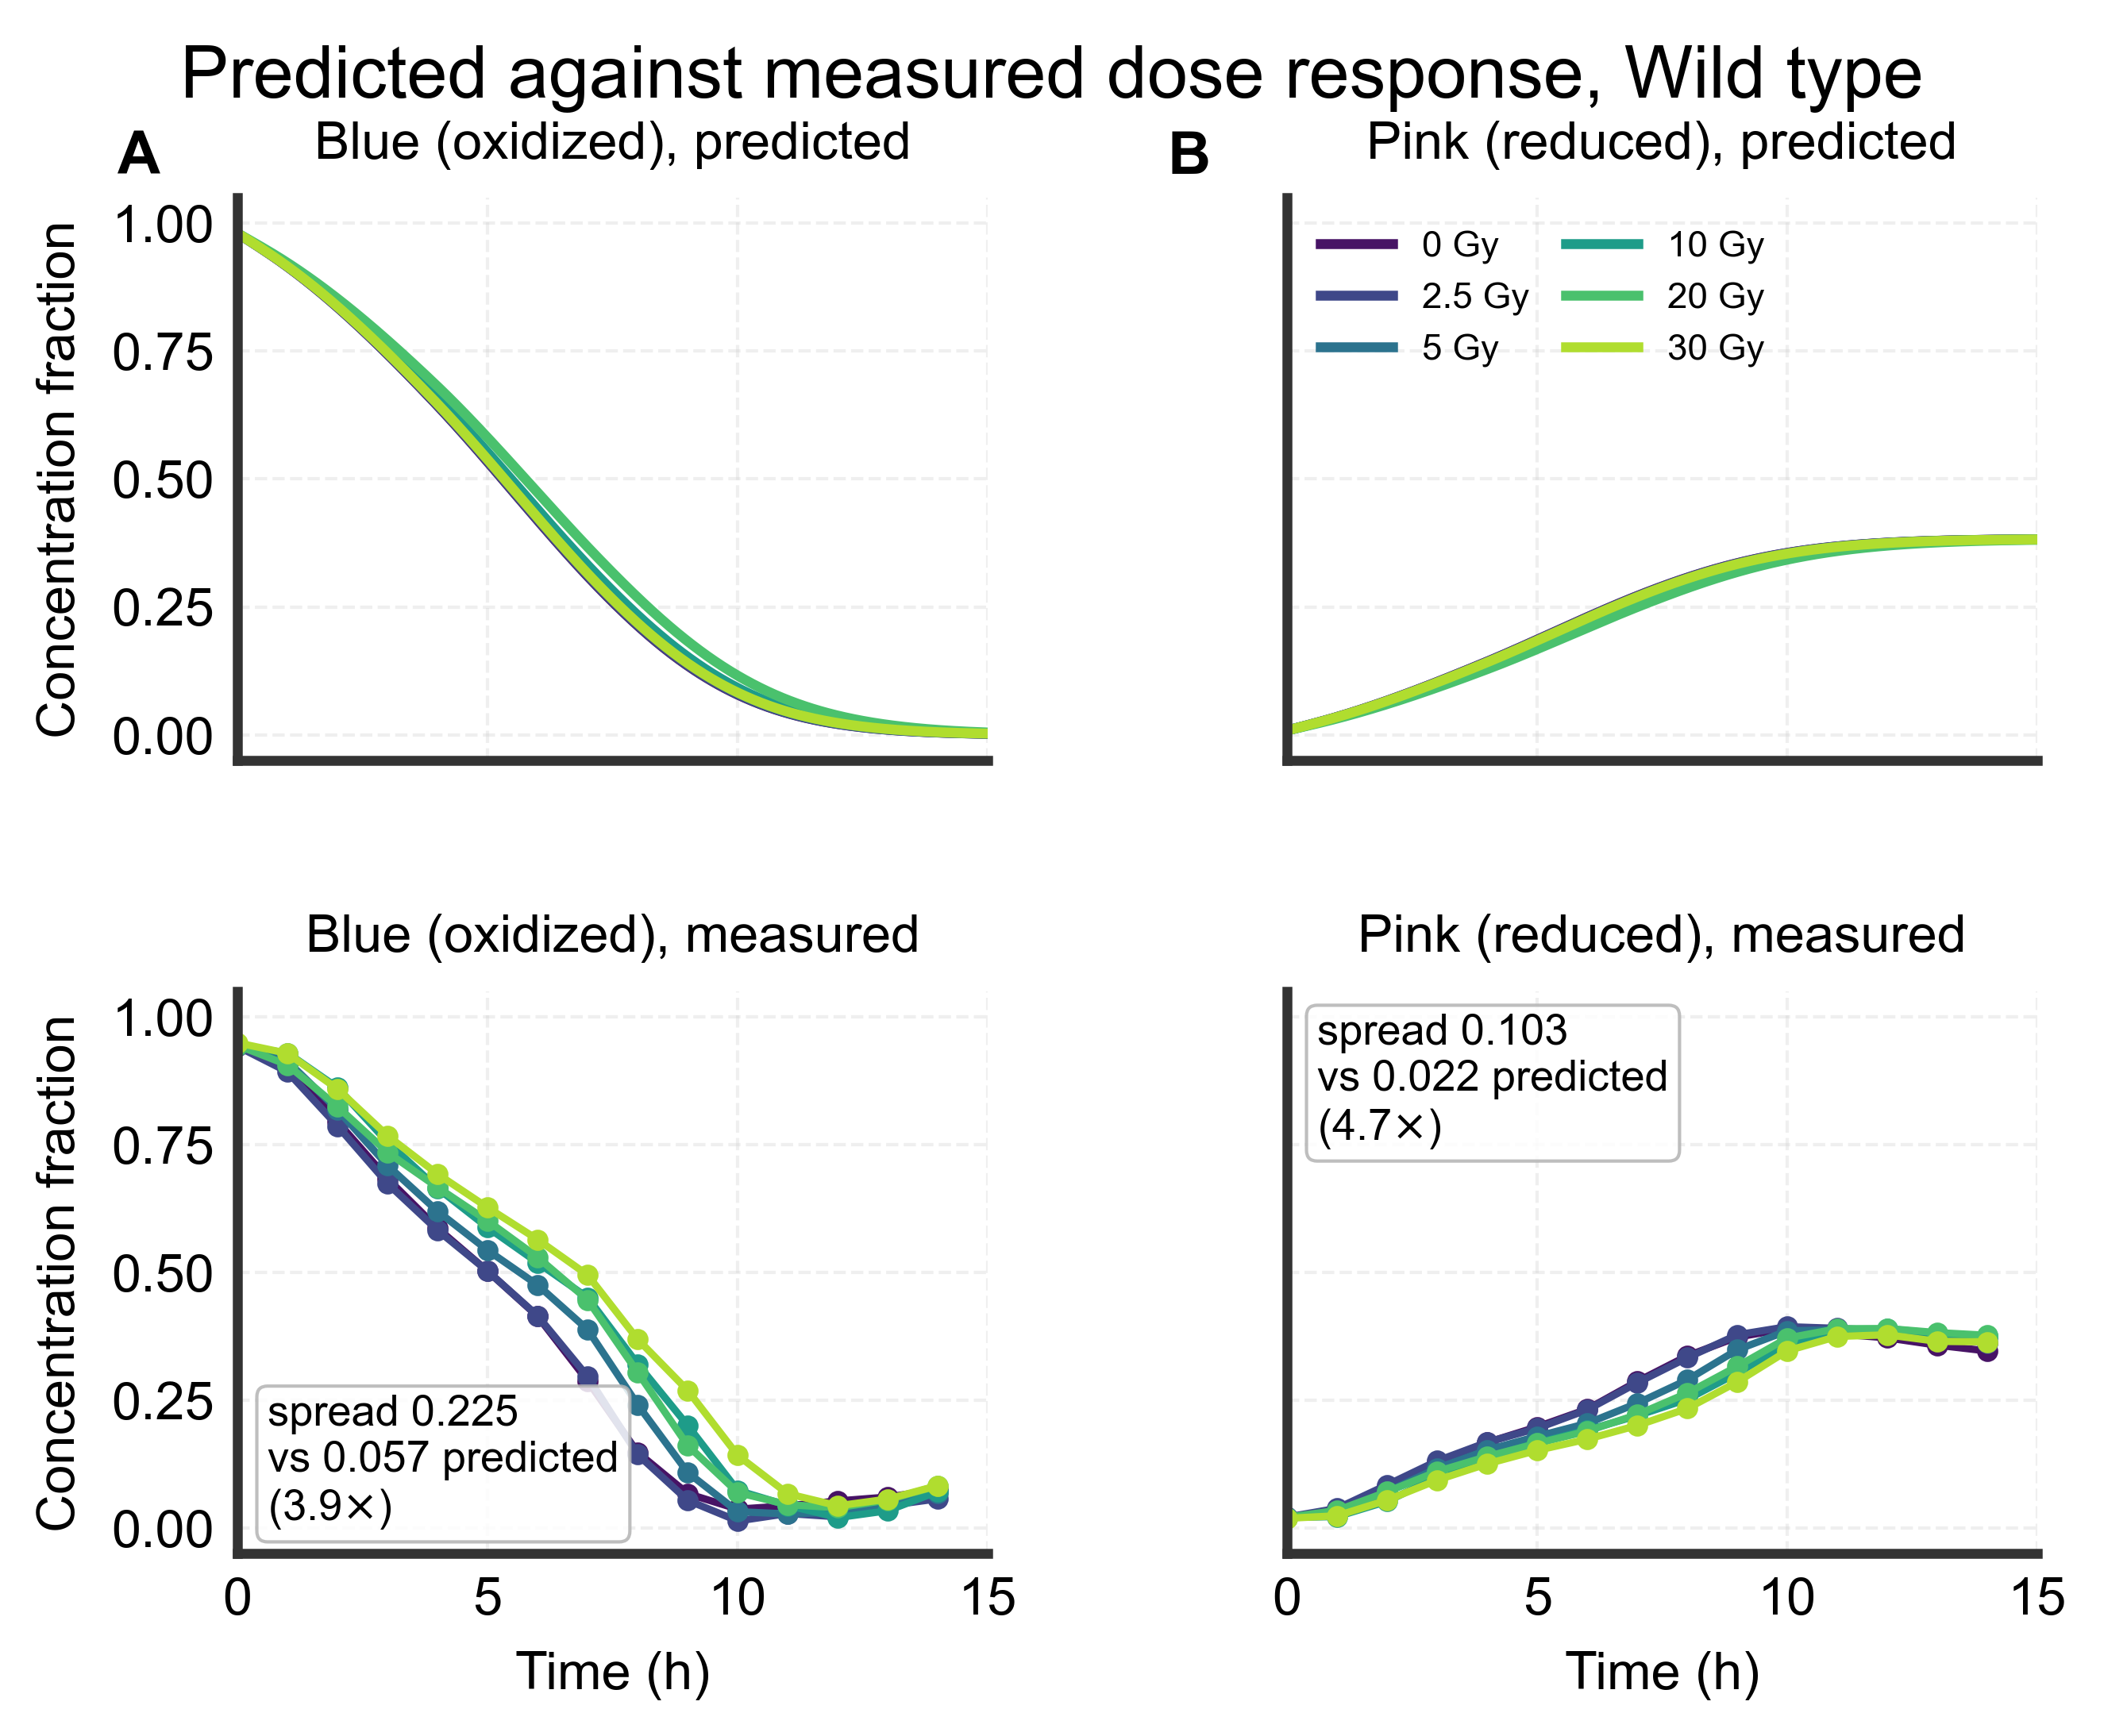
\includegraphics[width=0.9\textwidth]{Figures/ab_predicted_vs_measured_WT.png}
\end{center}
\caption{\textit{Corresponds to Results, ``AMMPER generates alamarBlue reduction curves using a naive Michaelis-Menten bulk model'' in the main text, where this figure is cited.} \textbf{Wild type.} Dose dependence of the predicted and measured aB response, with predictions (top row) and measurements (bottom row) on matched axes so that the two can be compared directly without rescaling. Dose is indicated by color; the left column shows the blue (oxidized) species and the right column the pink (reduced) species. Insets give the measured and predicted peak-to-peak spread across dose at the timepoint of greatest separation, and their ratio. The predicted and measured curves are ordered by dose in the same direction in both species, but the predicted separation is four- to fivefold smaller than the measured one (0.057 against 0.225 concentration-fraction units for the blue species, 0.022 against 0.103 for the pink). The compression originates in the narrow spread of the simulated population trajectories across dose rather than in the kinetic model, which is quantified in Fig.~\ref{fig:S4} and discussed in Supplementary Text S3. The corresponding figure for \textit{rad51}$\Delta$ is Fig.~\ref{fig:S2}.}
\label{fig:S1}
\end{figure}

% ---------- S2 : predictions against measurements, rad51-delta ----------
\begin{figure}[h!]
\begin{center}
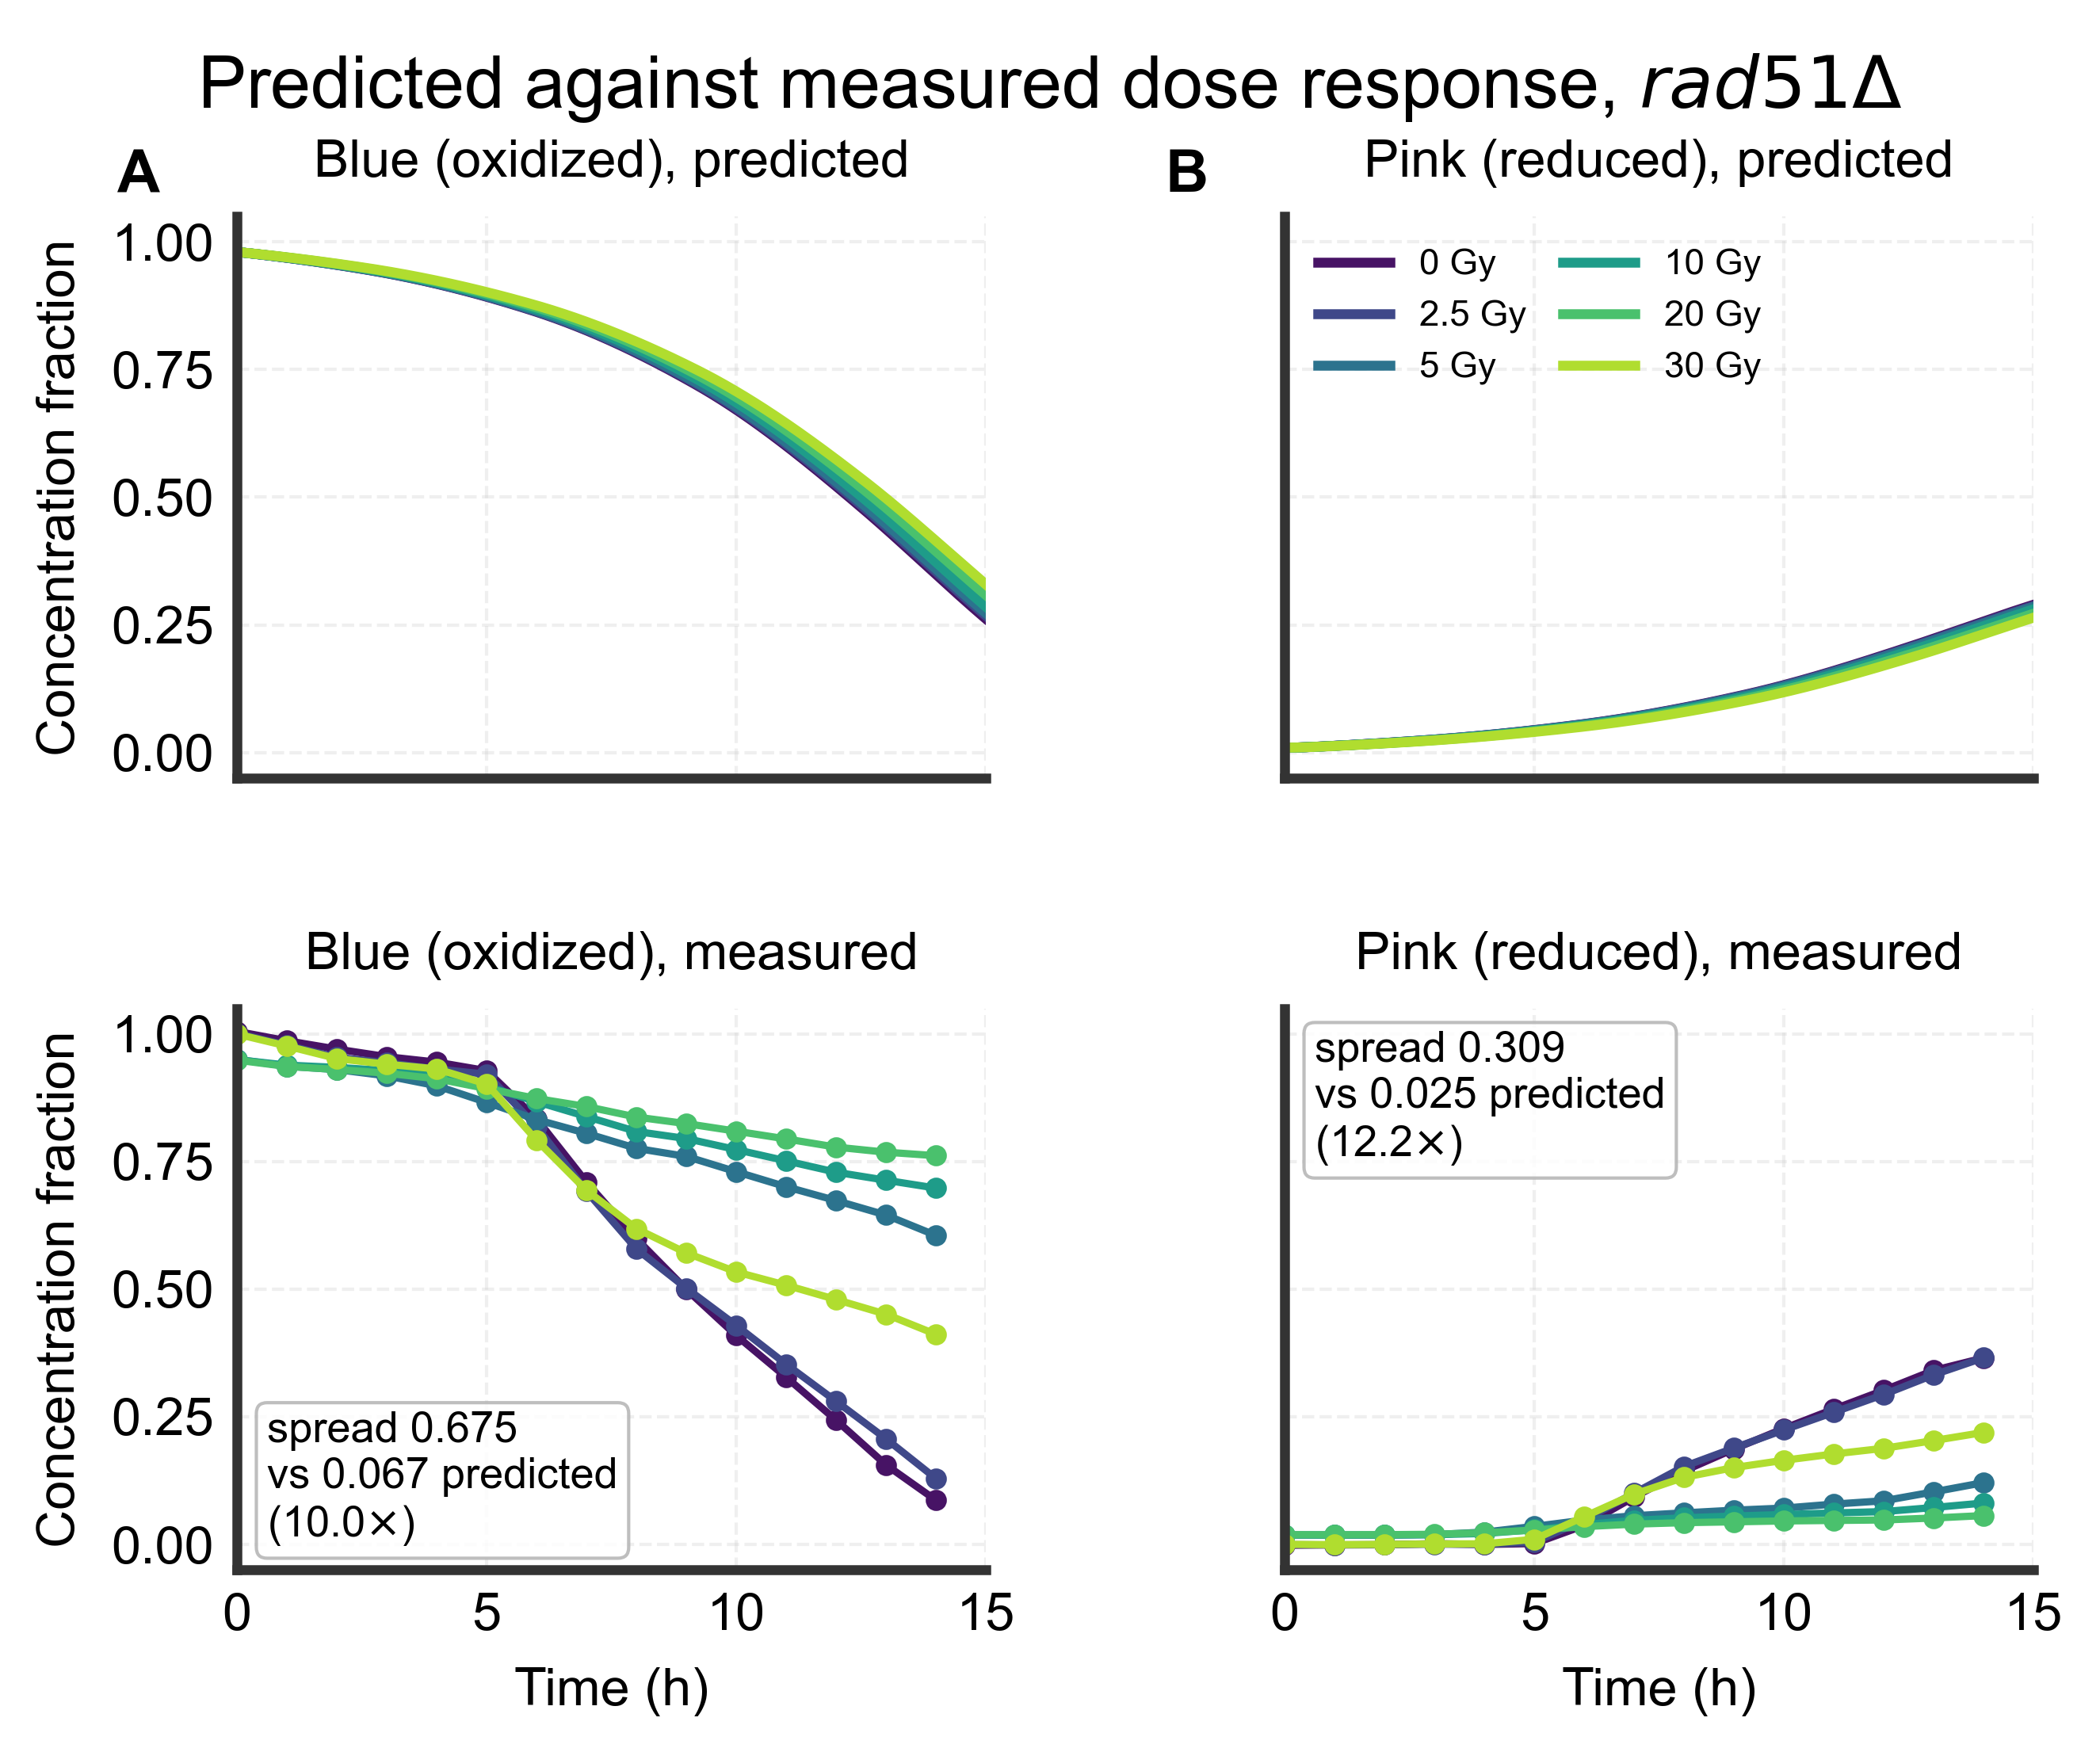
\includegraphics[width=0.9\textwidth]{Figures/ab_predicted_vs_measured_rad51.png}
\end{center}
\caption{\textit{Corresponds to Results, ``AMMPER generates alamarBlue reduction curves using a naive Michaelis-Menten bulk model'' in the main text, where this figure is cited.} \textbf{\textit{rad51}$\Delta$.} Dose dependence of the predicted and measured aB response, with predictions (top row) and measurements (bottom row) on matched axes so that the two can be compared directly without rescaling. Dose is indicated by color; the left column shows the blue (oxidized) species and the right column the pink (reduced) species. Insets give the measured and predicted peak-to-peak spread across dose at the timepoint of greatest separation, and their ratio. The predicted ordering is perfectly monotonic in dose (rank correlation $\pm 1.00$) whereas the measured curves are not, and the compression is correspondingly more severe: approximately tenfold for the blue species (0.067 against 0.675) and twelvefold for the pink (0.025 against 0.309). The compression originates in the narrow spread of the simulated population trajectories across dose rather than in the kinetic model, which is quantified in Fig.~\ref{fig:S4} and discussed in Supplementary Text S3. The corresponding figure for the wild type is Fig.~\ref{fig:S1}.}
\label{fig:S2}
\end{figure}

% ---------- S3 : Propagator distribution ----------
\begin{figure}[h!]
\begin{center}
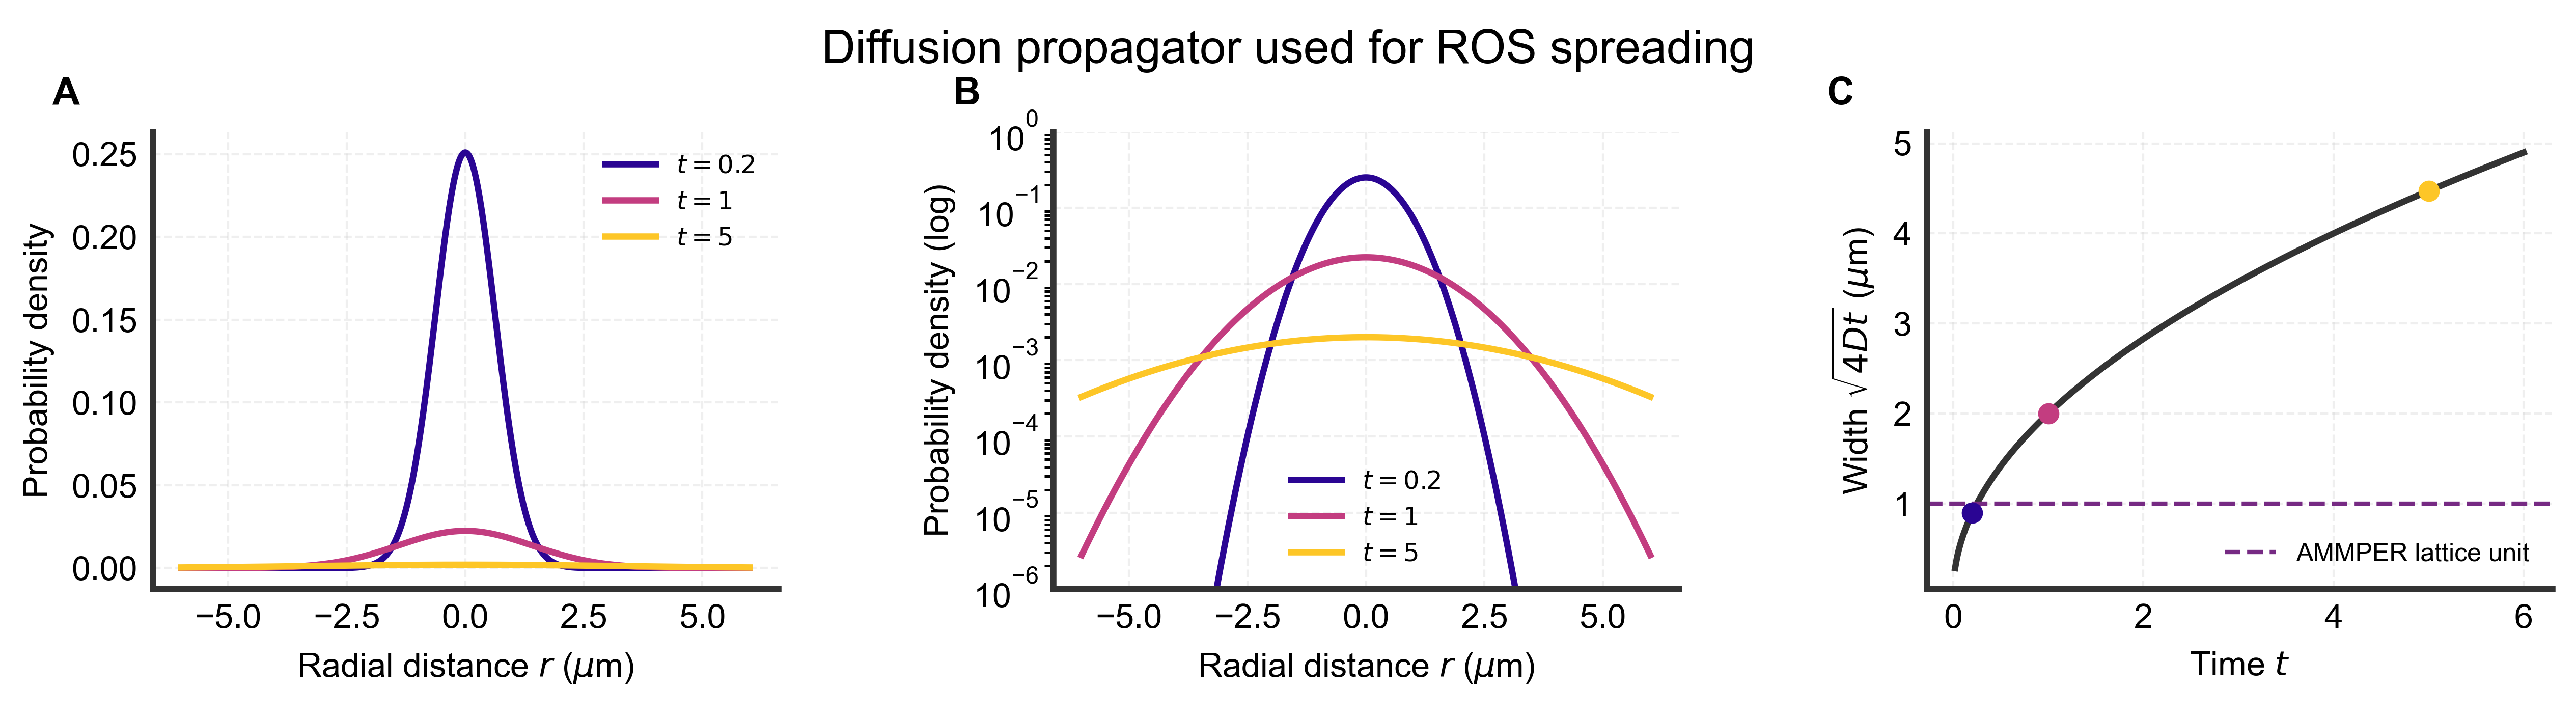
\includegraphics[width=0.95\textwidth]{Figures/diffusion_propagator.png}
\end{center}
\caption{\textit{Corresponds to Results, ``Implementing decay and diffusion of reactive oxygen species produces little benefit over the naive model'', and to Materials and Methods, ``Diffusion and decay ROS molecule modeling'', where this figure is cited.} Time evolution of the diffusion propagator (Equation~\ref{eq:S_prop}), evaluated along a radial line for visualization at three times ($t = 0.2$, $1$ and $5$ in the arbitrary units of the figure, with $D = 1$). \textbf{(A)} Linear density axis. The probability density broadens as material initially localized at a point source disperses, and the peak height falls as $t^{-3/2}$, a factor of 125 across the times shown. \textbf{(B)} The same three profiles on a logarithmic density axis, which is where the broadening is legible: on the linear axis the $t=5$ profile lies flat against zero. Both axes are shown because the linear panel is the faithful picture of relative magnitude and the logarithmic one the readable picture of shape. \textbf{(C)} The width $\sqrt{4Dt}$ implied by the propagator, with the three times marked and the AMMPER lattice spacing shown as a dashed line. Spreading narrower than one lattice unit cannot be represented on the discrete grid, which sets the shortest interval over which the diffusion model differs from the naive one.}
\label{fig:S3}
\end{figure}

% ---------- S4 : Non-parametric damage distribution ----------
\begin{figure}[h!]
\begin{center}
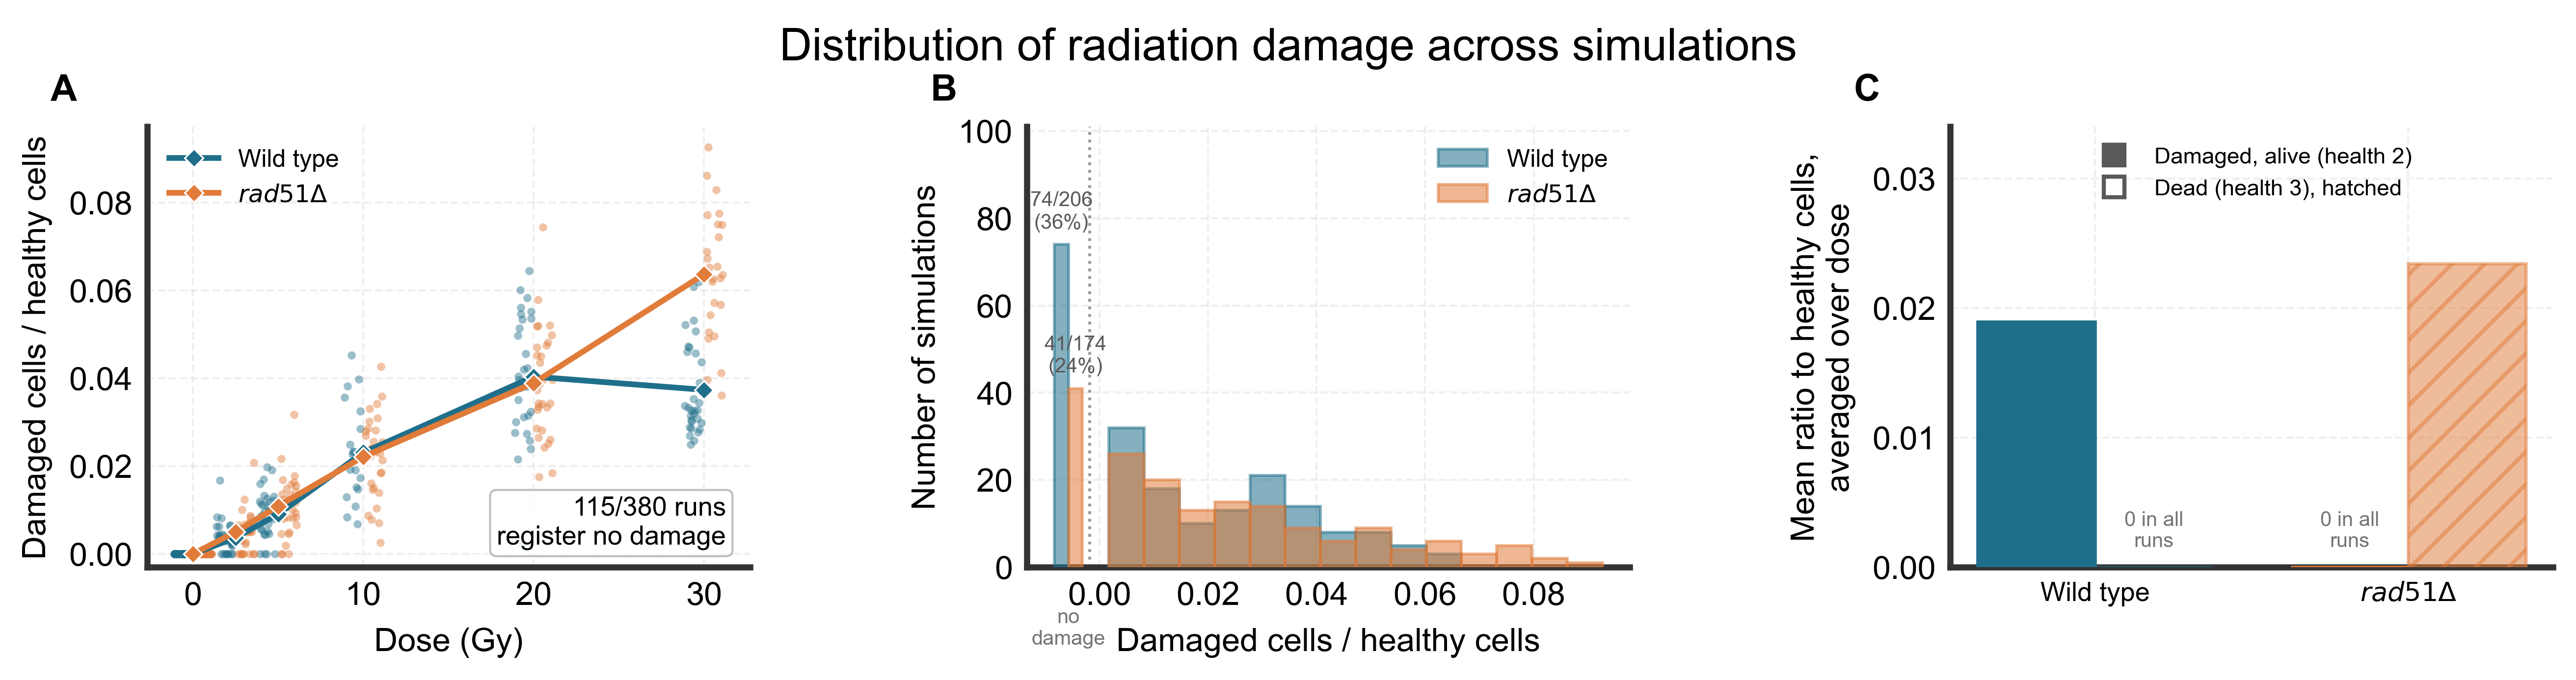
\includegraphics[width=0.95\textwidth]{Figures/damage_distribution.png}
\end{center}
\caption{\textit{Corresponds to Results, ``AMMPER generates alamarBlue reduction curves using a naive Michaelis-Menten bulk model'' and ``Variance among AMMPER simulations is associated with localization of damage from ion tracks'', where this figure is cited.} Distribution of radiation damage across all 380 archived proton simulations. \textbf{(A)} Per-run ratio of damaged to healthy cells at the end of the run, against dose, with every run plotted (horizontal jitter and a per-strain offset only; the vertical values are unperturbed) and the per-dose mean overlaid. 115 of the 380 runs register no damage at all. 92 of those are the two unirradiated 0~Gy conditions, which record no damage by construction; the remaining 23 are irradiated runs, 8 of 32 and 4 of 30 in the wild type and 8 of 29 and 3 of 30 in \textit{rad51}$\Delta$ at 2.5 and 5~Gy respectively, in which the ion track --- placed randomly at generation 2, when the population is four cells --- missed the population. No run at 10~Gy or above, in either strain, is free of damage. The distribution is therefore zero-inflated and strongly non-normal, which is the justification for the rank-based tests used in the main text. \textbf{(B)} The same runs as a histogram of the per-run damage ratio, pooled over dose, one series per strain. The runs with no damage at all are drawn as separate bars to the left of the dotted break, labeled with their counts (74 of 206 wild type runs, 41 of 174 in \textit{rad51}$\Delta$), so that they are not pooled with runs carrying small nonzero ratios; the bars to the right of the break are the nonzero runs only. The distribution is therefore zero-inflated, with a short right tail and no central mode, which is why the analyses reported in the main text use rank-based rather than parametric tests. \textbf{(C)} The two damage states separately, averaged over dose. Each strain has exactly one nonzero bar, and the state that is empty in every run of that strain is annotated as such rather than drawn as a zero-height bar: the wild type accumulates cells in the damaged-but-alive state (health 2) and never a dead cell in any of 206 runs, while \textit{rad51}$\Delta$ accumulates dead cells (health 3) and never a damaged-but-alive one in any of 174. This is a property of the implementation rather than of the data: \texttt{cellROS\_rad51} assigns any damaged mutant cell directly to the nonviable state, so the mutant has no repairable-damage state by construction. It is the binary health-state limitation identified in the Discussion, made quantitative. Even at the highest dose the damage ratio remains small (mean 0.037 for the wild type at 30~Gy and 0.064 for the mutant), which is the origin of the compressed dose separation in Fig.~\ref{fig:S1}.}
\label{fig:S4}
\end{figure}

% ---------- S5 : Run-time comparison, re-measured ----------
\begin{figure}[h!]
\begin{center}
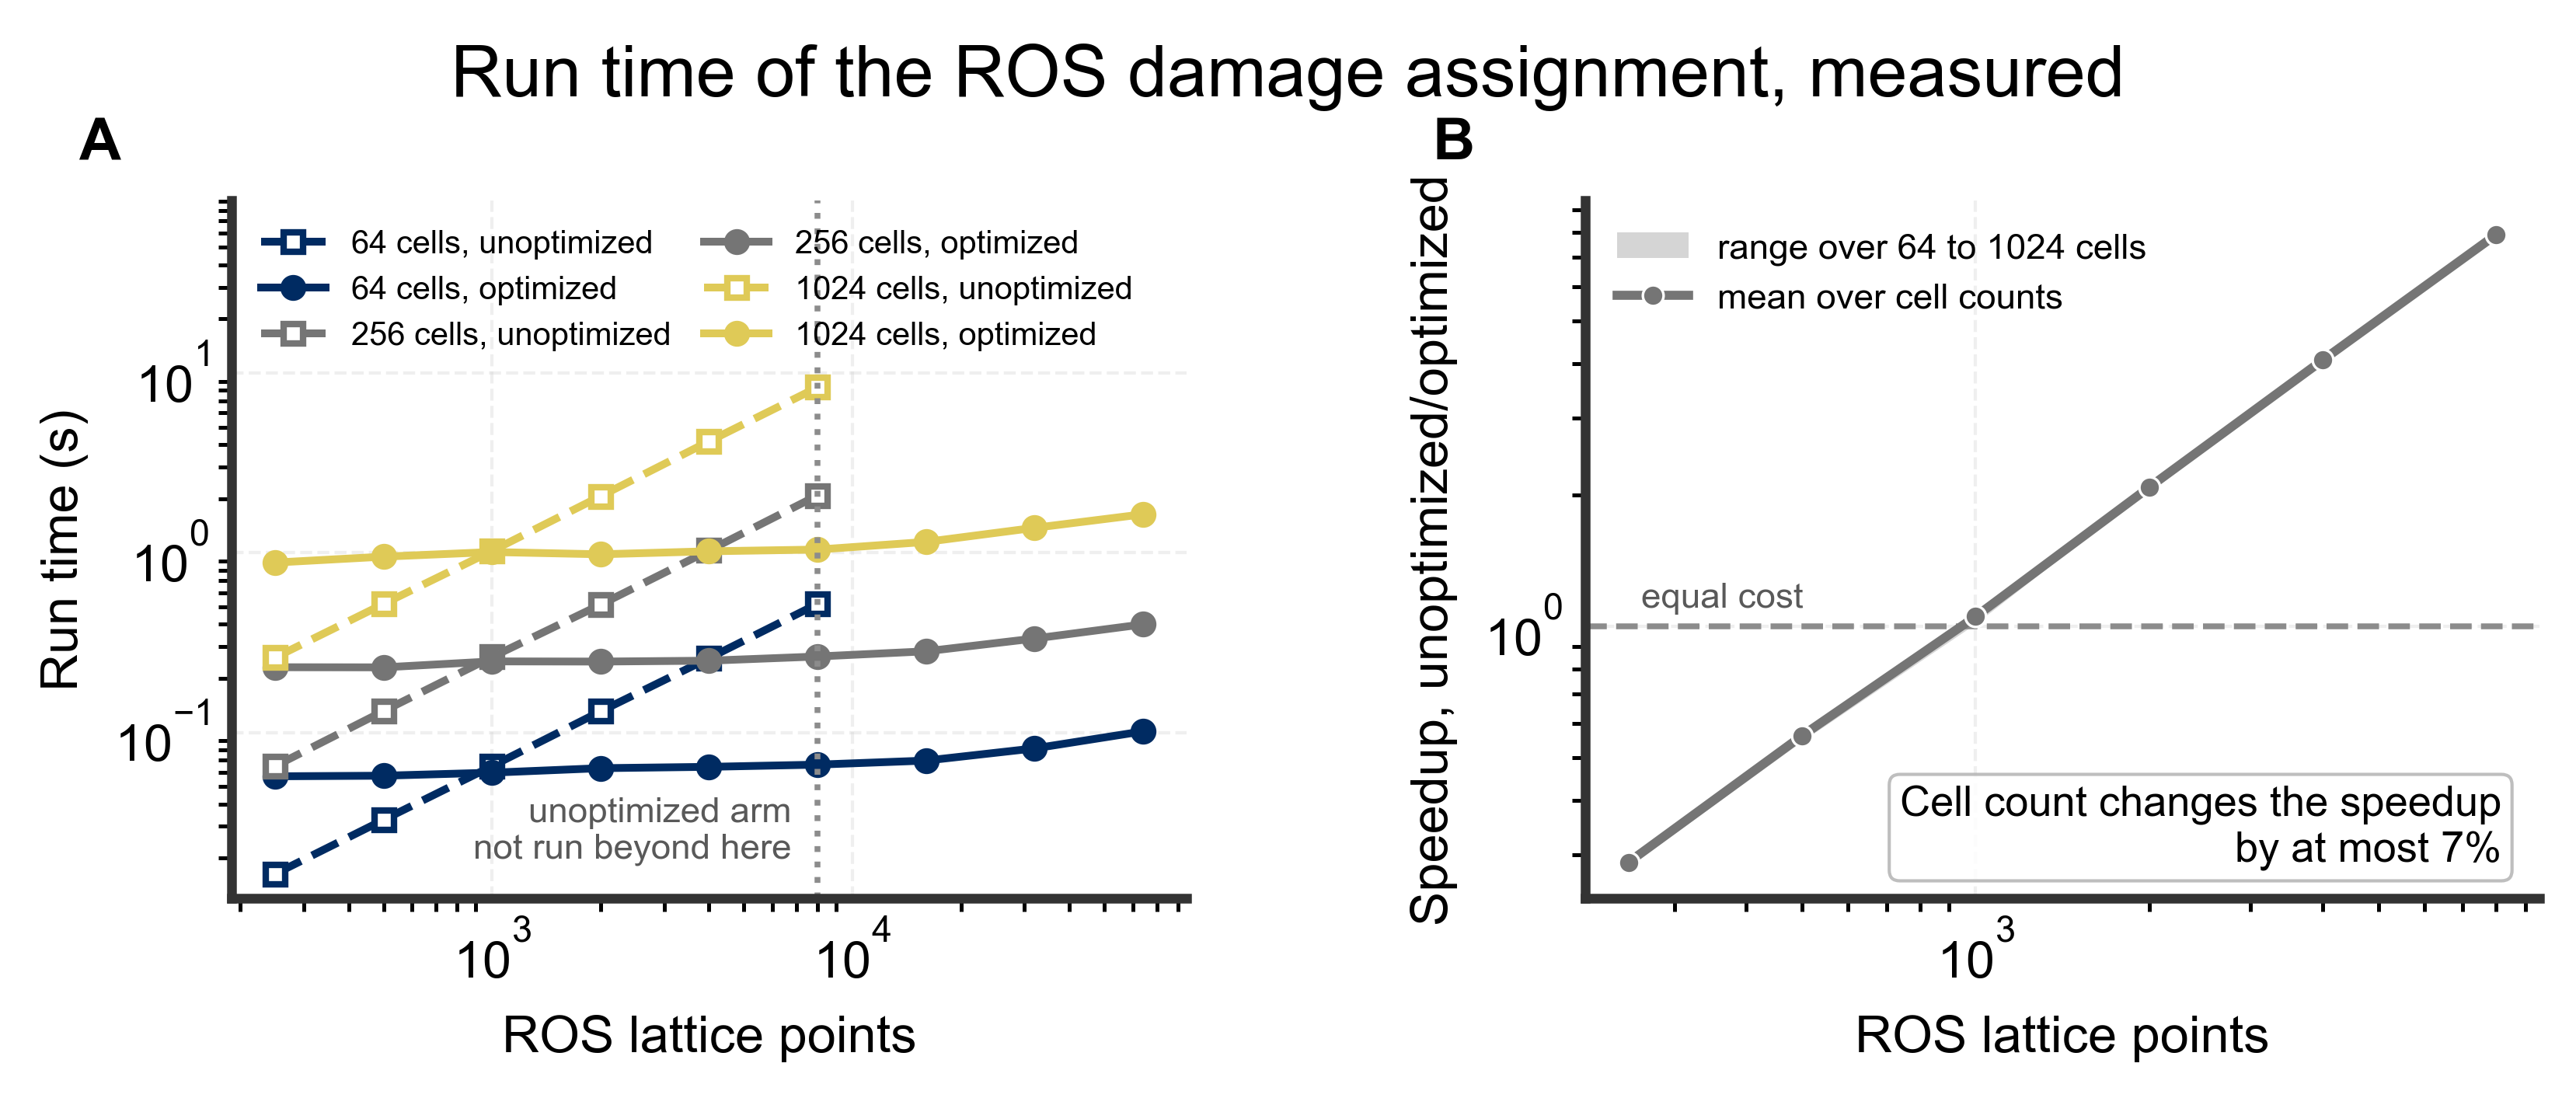
\includegraphics[width=0.95\textwidth]{Figures/ros_optimization.png}
\end{center}
\caption{\textit{Corresponds to Results, ``AMMPER-2 requires reduced computational resources due to optimization of visualization process and ROS damaging mechanics'', where this figure is cited.} Measured run time of the two ROS damage-assignment implementations, on identical inputs whose hit counts are asserted equal so that the comparison is of two implementations of one operation. ``Unoptimized'' is the interpreted nested loop over every ROS--cell pair used in AMMPER-1; ``optimized'' is the vectorized bounding-box filter used in AMMPER-2. Each point is the minimum of three repeats. \textbf{(A)} Run time against the number of ROS lattice points, for 64, 256 and 1024 cells. The unoptimized arm was not run beyond 8{,}000 points, marked by the dotted line, and the curve stops there rather than being extrapolated. \textbf{(B)} The ratio of the two, on the measured range. The vectorized implementation is slower below about 1{,}000 points, where a per-call filter overhead is not amortized, and faster above it by a factor that grows with problem size, reaching 8.0$\times$ at 8{,}000 points. This is the regime that matters in practice, since the diffusion ROS model emits 82 lattice points per deposition event where the naive model emits one, so enabling diffusion moves a simulation well to the right of the crossover. Measured on Linux 6.12.94 (x86\_64), Python 3.12.13, NumPy 1.26.4, pandas 2.3.3.}
\label{fig:S5}
\end{figure}

% WITHDRAWN from the supplement, this revision round: the SMAC3 Bayesian
%   optimization convergence figure (smac_convergence). SMAC3 was the optimizer of
%   the earlier version of this pipeline and is not what produced any number
%   reported in this work; every reported parameter comes from the differential
%   evolution search in fit_ab_model_fixed.py. The figure and its narrative are
%   removed so that the manuscript describes only the fit that was actually run.
%   The plotting code remains in make_supplementary_figures.py and the SMAC run
%   archives remain in the repository, so it can be reinstated if a reviewer asks
%   how the two searches compare.

% ---------- S6 : AMMPER visualizations, gamma vs ion track ----------
\begin{figure}[h!]
\centering
\begin{subfigure}[b]{0.48\textwidth}
\centering
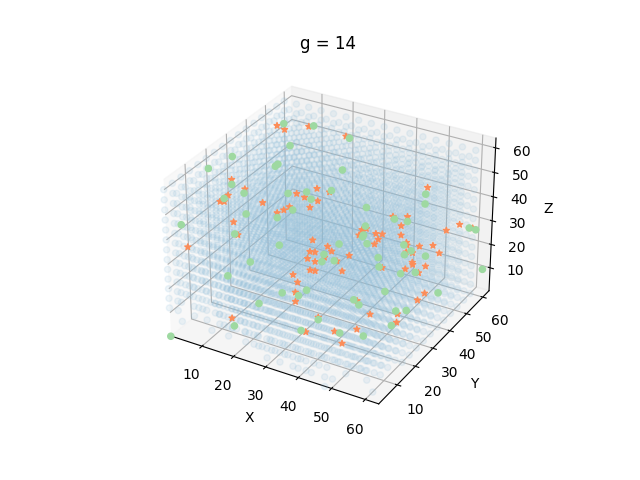
\includegraphics[width=\linewidth]{Figures/AMMPERgamma.png}
\caption{Gamma radiation AMMPER visualization with \textit{rad51}$\Delta$ cells.}
\label{fig:S6a}
\end{subfigure}
\hfill
\begin{subfigure}[b]{0.48\textwidth}
\centering
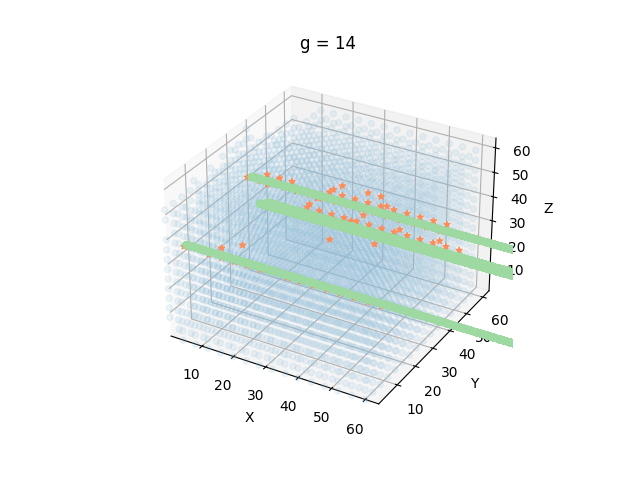
\includegraphics[width=\linewidth]{Figures/AMMPERiontrack.png}
\caption{Ion track AMMPER visualization, 150 MeV at 15 Gy, \textit{rad51}$\Delta$ cells.}
\label{fig:S6b}
\end{subfigure}
\caption{\textit{Corresponds to Supplementary Text S2, where this figure is cited.} AMMPER visualizations with \textit{rad51}$\Delta$ cells. Healthy cells are depicted as blue circles, dead cells as red circles, and green circles or tracks represent the initial positions of ROS molecules generated by radiation events. \textbf{(a)} Gamma radiation causes non-localized damage to the cell population. \textbf{(b)} Ion tracks result in localized ROS generation along the tracks, with dead cells shown in red around the tracks. Healthy yeast cells, depicted in blue, are rarely affected if they are far from the tracks. This contrast in damage topology is what makes the gamma environment a distinct test of the model rather than a repeat of the proton one; its consequence for the simulated population is quantified under ``Why gamma is worth reporting alongside protons'' in Text S2.}
\label{fig:S6}
\end{figure}

% ---------- S7 : Gamma aB predictions, both strains ----------
% Sized to fit one page: the two 0.59-aspect blocks at 0.75\textwidth occupy about
% 4.7in of the 9in text height, leaving room for this figure's long caption. At
% 0.9\textwidth they overfull the page and the float moves past its callout.
% [p] rather than [h!] for the same reason -- a full-page float is what this is.
\begin{figure}[p]
    \centering
    \begin{subfigure}[b]{0.75\textwidth}
        \centering
        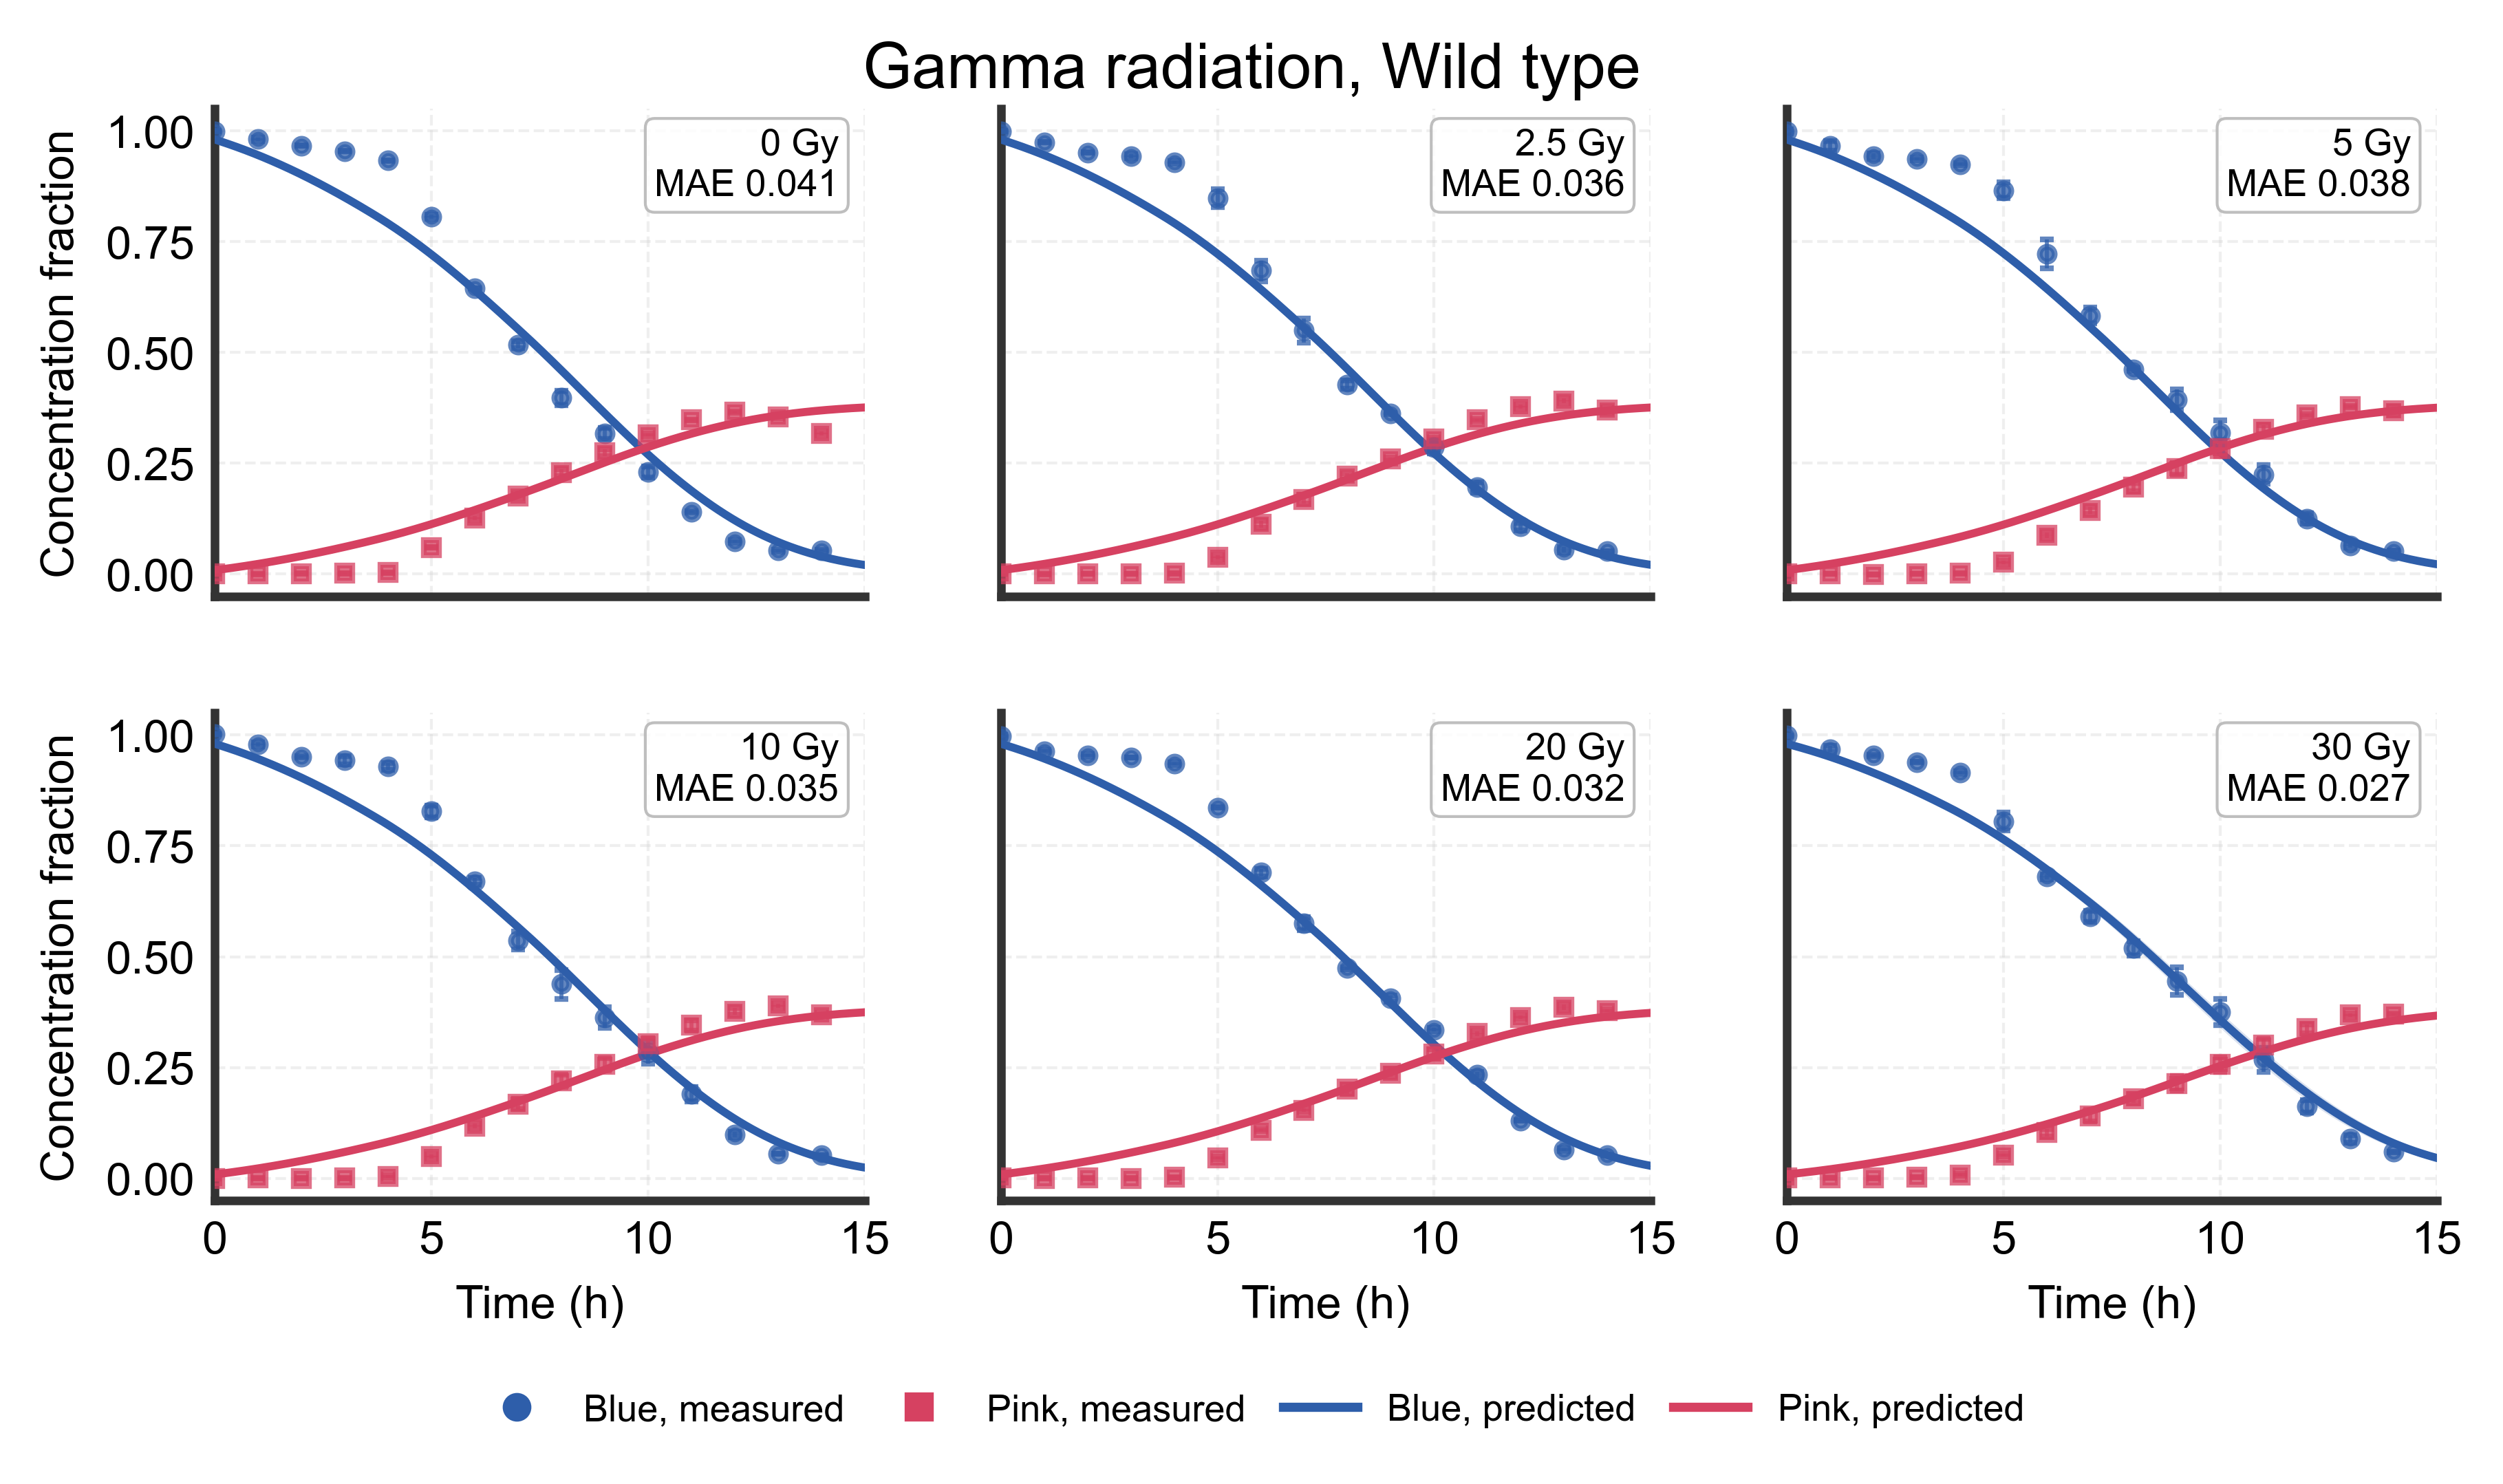
\includegraphics[width=\linewidth]{Figures/gamma_ab_predictions_WT.png}
        \caption{Wild type}
        \label{fig:S7a}
    \end{subfigure}
    \\[0.5em]
    \begin{subfigure}[b]{0.75\textwidth}
        \centering
        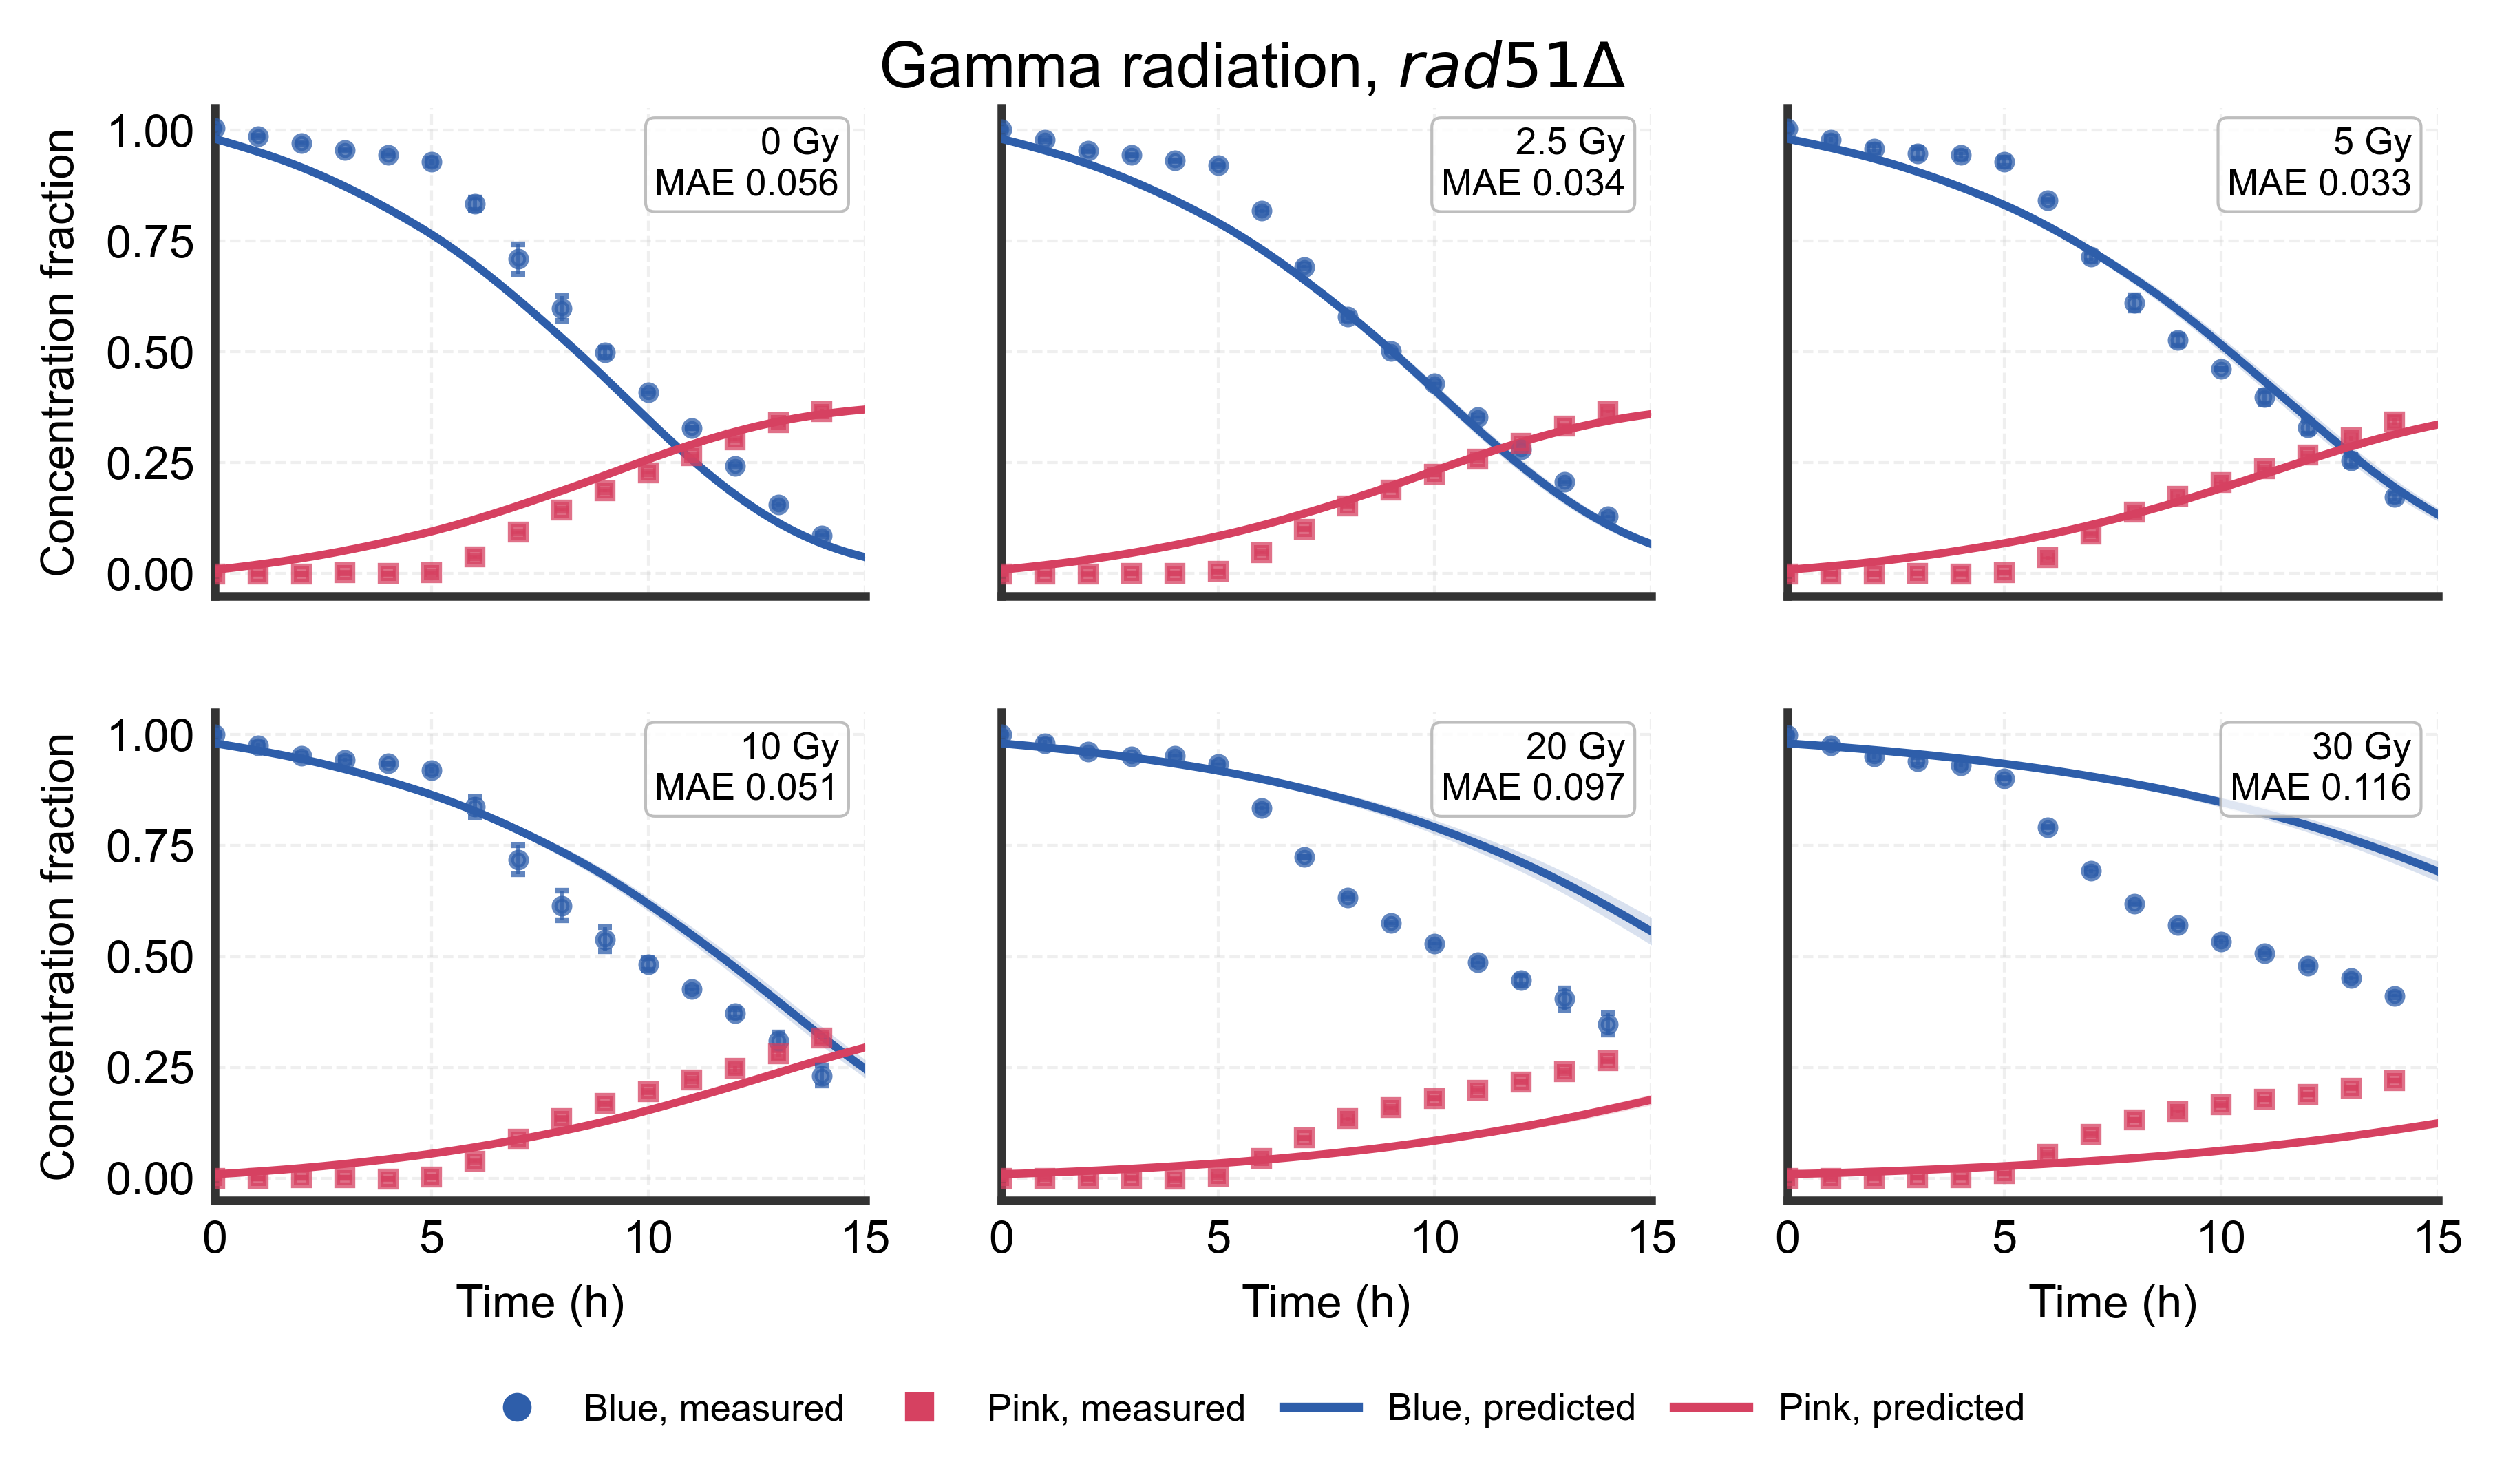
\includegraphics[width=\linewidth]{Figures/gamma_ab_predictions_rad51.png}
        \caption{\textit{rad51}$\Delta$}
        \label{fig:S7b}
    \end{subfigure}
    \caption{\textit{Corresponds to Results, ``The aB model transfers to a gamma radiation environment'', and to Supplementary Text S2, where this figure is cited.} Predicted and measured aB response under gamma radiation, one axes per dose, laid out to match main-text Figure~2 so that the two radiation qualities can be compared without rescaling. Points with error bars are the measurements; lines are the mean over the replicate simulations for that condition with the shaded band giving the standard error of that mean. Twelve replicates are used for each irradiated condition, rather than three, because at the calibrated hit rate the number of deposition events per plane is small (5 at 2.5~Gy, 56 at 30~Gy) and which cells are struck is correspondingly stochastic; the two 0~Gy conditions reuse the unirradiated proton archives, in which no radiation is applied. The inset in each axes gives the dose and the mean absolute error. The kinetic constants are transferred unchanged from the proton fit and only the inoculum offset $g_0$ is refit per strain. \textbf{(a)} Wild type, mean absolute error 0.035, uniform across dose (0.026--0.041). \textbf{(b)} \textit{rad51}$\Delta$, mean absolute error 0.064, with the residual concentrated at the two highest doses (0.096 at 20~Gy and 0.116 at 30~Gy) where the measured curves flatten toward dose-dependent plateaus that the model cannot produce. Over all twelve conditions the mean absolute error is 0.049, against 0.051 for the twelve proton conditions.}
    \label{fig:S7}
\end{figure}

% WITHDRAWN from the supplement at the authors' discretion, this revision round:
%   the gamma hit-rate calibration figure (gamma_hit_rate_calibration) and the
%   gamma-against-proton comparison (gamma_vs_proton). Both remain in the code
%   (make_gamma_figures.py) and both are regenerated by it, so either can be
%   reinstated if a reviewer asks for it. The numbers each carried are stated in
%   Supplementary Text S2 instead, which is where they are cited from.

\clearpage

% =====================================================================
\bibliographystyle{unsrt}
\bibliography{references}
% =====================================================================

\end{document}
